\chapter{METODOLOGI}

% Ubah konten-konten berikut sesuai dengan isi dari metodologi
Bab ini menguraikan tahapan sistematis dan metode yang diterapkan dalam melaksanakan penelitian tugas akhir ini. Penjelasan mencakup rancangan kerangka sistem asesmen kepribadian yang menggunakan pendekatan hibrida, mulai dari tahap pemrosesan data visual hingga pengujian hasil akhir. Bab ini juga merinci metode pendekatan yang digunakan, bahan dan peralatan pendukung eksperimen, serta teknis urutan pelaksanaan penelitian secara keseluruhan.

\section{Metode yang digunakan}

Bagian ini menguraikan rangkaian metode yang diterapkan untuk mengekstraksi dan menginterpretasi profil kepribadian \textit{Big Five} berdasarkan fitur visual dari potongan video. Berdasarkan \autoref{fig:flowchart-penelitian}, tahapan penelitian diawali dengan praproses dataset video menjadi kumpulan gambar statis yang dilanjutkan dengan proses prediksi serta evaluasi nilai numerik kepribadian. Alur tersebut kemudian memasuki tahap perancangan \textit{prompt}, interpretasi kepribadian menggunakan LLM, dan evaluasi akhir terhadap kualitas narasi yang dihasilkan.

\begin{figure}[H]
	\centering
	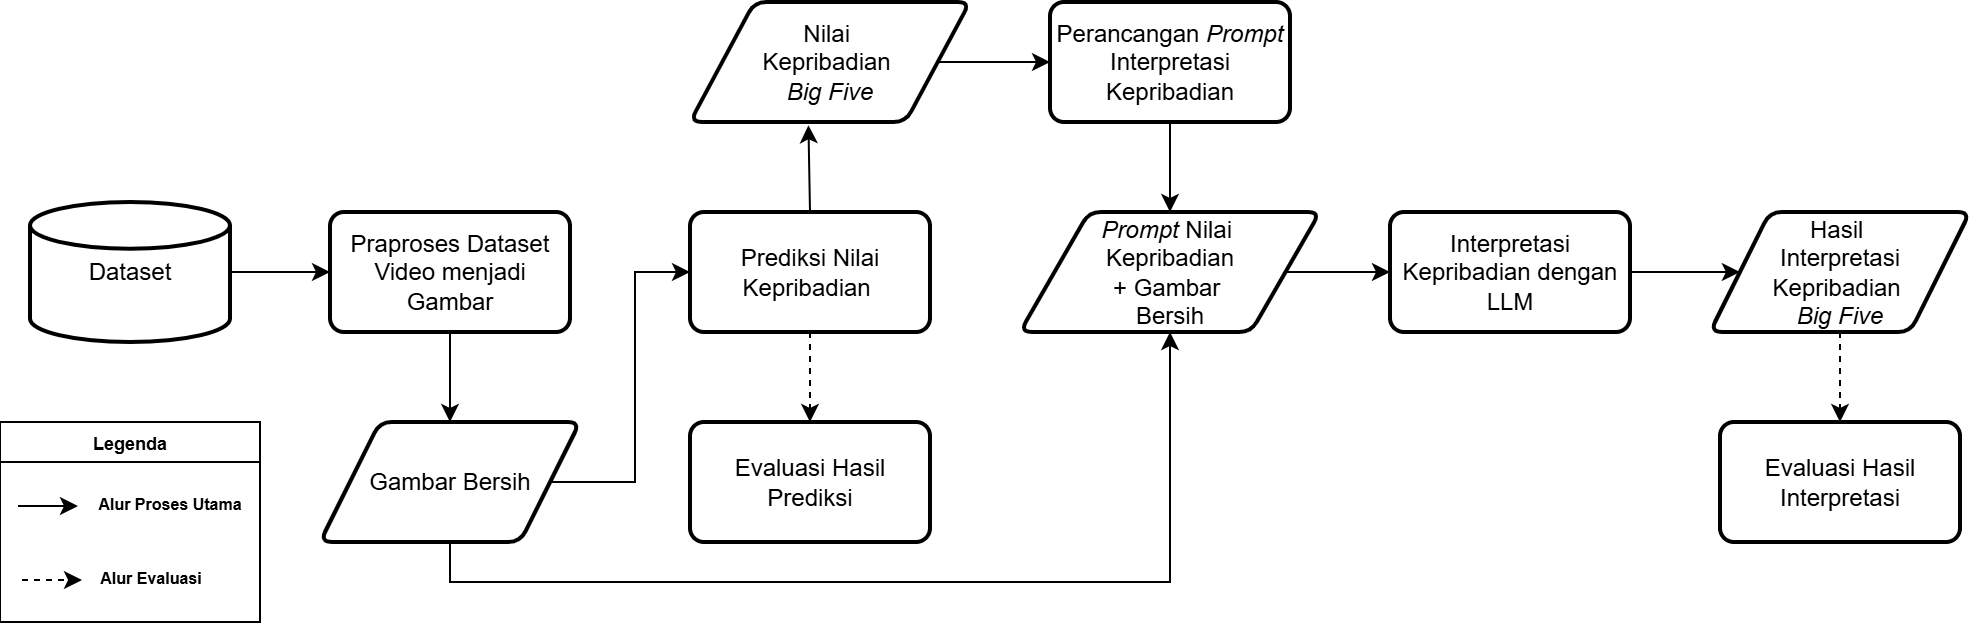
\includegraphics[width=\linewidth]{gambar/flowchart-penelitian.png}
	\caption{Diagram Alir Penelitian}
	\label{fig:flowchart-penelitian}
\end{figure}

\subsection{Praproses Dataset Video menjadi Gambar}
\label{subsec:praproses-dataset}

Dataset ChaLearn yang digunakan merupakan dataset dengan modalitas video. Oleh karena itu, diperlukan konversi data menjadi gambar statis. Setiap \textit{frame} yang diekstraksi dari video diperlakukan sebagai satu sampel data tunggal yang independen. Tahapan praproses dilakukan untuk mentransformasi data mentah ke dalam format visual yang terstandarisasi sebelum dipelajari oleh model prediksi. Rangkaian keseluruhan dari proses transformasi data ini ditunjukkan secara visual melalui diagram alir pada \autoref{fig:flowchart-praproses}. Untuk menghasilkan kualitas input yang optimal bagi model, terdapat serangkaian langkah praproses yang dieksekusi secara berurutan sebagai berikut:

\begin{enumerate}[nosep]
	\item Ekstraksi \textit{frame} dan pelabelan gambar dilakukan untuk mengubah data video menjadi gambar statis. Dilakukan pengambilan sampel \textit{frame} sebanyak 15 dengan interval tetap dari setiap video dalam dataset untuk mewakili setiap detik dalam video yang rata-rata berdurasi 15 detik. Setiap \textit{frame} yang diekstraksi diberi label yang sama dengan video induknya. Sebagai contoh, jika sebuah video memiliki nilai \textit{Openness} 0.8, maka seluruh gambar yang diekstraksi dari video tersebut akan dilabeli dengan nilai \textit{Openness} 0.8. Hal ini memungkinkan model untuk belajar mengasosiasikan fitur visual statis sesaat dengan label kepribadian secara keseluruhan.

	\item Deteksi wajah utama dan \textit{cropping} dilakukan karena fokus penelitian adalah \textit{apparent personality} dari wajah manusia, maka tampilan latar belakang yang tidak relevan dihilangkan. MediaPipe \textit{Face Detection} digunakan untuk mendeteksi wajah, kemudian dilakukan \textit{cropping} pada gambar berdasarkan \textit{bounding box} wajah yang terdeteksi dengan penambahan sedikit margin untuk memastikan seluruh fitur wajah seperti rambut tetap terlihat.

	\item Pengubahan ukuran dilakukan agar dimensi gambar sesuai dengan spesifikasi \textit{input} model prediksi, yaitu $224 \times 224$ untuk model ViT dan PVT, serta $256 \times 256$ untuk model Swin Transformer.
	
	\item Augmentasi dilakukan untuk memperkaya variasi gambar pada dataset, mengingat terdapat beberapa \textit{frame} yangmemiliki kemiripan karena hasil ekstraksi 15 \textit{frame} pada satu video. Augmentasi yang dilakukan meliputi \textit{Random Horizontal Flip} dengan probabilitas 0.5, \textit{Random Rotation} sebesar 10 derajat, dan mengubah kecerahan dan kontras gambar secara acak dengan faktor maksimal sebesar 0.2.
	
	\item Normalisasi dilakukan nilai piksel menggunakan normalisasi Z-\textit{score} dengan rata-rata untuk setiap \textit{channel} warna pada gambar $R=0.485$, $G=0.456$, dan $B=0.406$ serta standar deviasi untuk setiap \textit{channel} secara berurutan $0,229$, $0,224$, dan $0,225$. Nilai ini didapatkan dari perhitungan dataset ImageNet yang digunakan untuk pelatihan awal model \textit{pretrained} Transformer yang selanjutnya dilatih menggunakan dataset ChaLearn untuk menyesuaikan kebutuhan prediksi kepribadian.
\end{enumerate}

\begin{figure}[H]
	\centering
	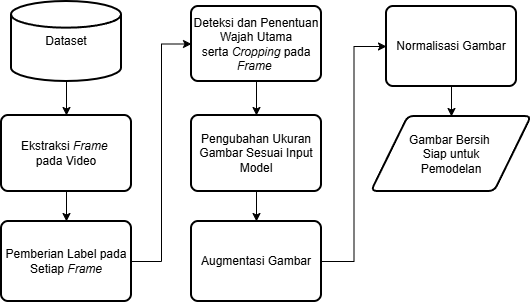
\includegraphics[width=0.7\linewidth]{gambar/flowchart-praproses.png}
	\caption{Diagram Alir Praproses Dataset}
	\label{fig:flowchart-praproses}
\end{figure}

\subsection{Arsitektur Model Regresi Transformer}
\label{subsec:arsitektur-regresi-bigfive}
Penelitian ini memanfaatkan arsitektur Transformer sebagai (\textit{backbone}) untuk ekstraksi fitur visual dari citra wajah. Tiga varian model digunakan untuk dibandingkan kinerjanya, yaitu ViT, Swin Transformer V2, dan PVT V2. Ketiga model ini merupakan model yang telah dilatih sebelumnya (\textit{pretrained}) pada dataset ImageNet untuk tugas klasifikasi gambar.

Adaptasi utama yang dilakukan dalam penelitian ini adalah mengubah fungsi model dari klasifikasi menjadi regresi multi-target (multi-target regression). Umumnya model-model tersebut memiliki lapisan akhir (\textit{head}) berupa lapisan linier (\textit{fully connected layer}) dengan ribuan neuron \textit{output} sesuai dengan jumlah kelas klasifikasi yang diikuti oleh fungsi aktivasi \textit{softmax}. Struktur ini tidak relevan untuk prediksi nilai kepribadian yang bersifat kontinu. Arsitektur model dirancang menggunakan dua komponen utama, yaitu \textit{backbone} dan \textit{regression head}. Visualisasi arsitektur ini dapat dilihat pada Gambar \ref{fig:custom-transformer-arch}. Berikut adalah penjelasan bagian dari arsitektur.

\begin{enumerate}[nosep]
	\item \textit{Backbone} Transformer, bagian ini menggunakan \textit{pre-trained} Transformer ViT, Swin V2, dan PVT V2. \textit{Backbone} ini bertugas mengubah citra \textit{input} menjadi representasi vektor global dengan dimensi $D$, di mana $D$ bergantung pada varian model yang digunakan.
	
	\item \textit{Custom regression head}, bagian ini berfungsi untuk mengadaptasi model Transformer yang umumnya digunakan untuk klasifikasi. Berbeda dengan \textit{head} klasifikasi standar, \textit{head} ini dirancang khusus untuk tugas regresi \textit{multi-output}. Komponen ini terdiri dari lapisan linear \textit{fully connected} dengan matriks \textit{weight} $W \in \mathbb{R}^{D \times 512}$, yang memetakan vektor fitur $D$ ke 512 neuron \textit{output} untuk memadatkan vektor fitur \textit{backbone} Transformer. \textit{Output} ini kemudian melewati \textit{hidden layer} \textit{Gaussian Error Linear Units} (GELU) untuk memetakan fitur non linear pada \textit{regression head}. Dibandingkan dengan ReLU, GELU bersifat \textit{smooth} dan probabilistik yang mengakomodasi nilai yang lebih kecil atau negatif sehingga menciptakan gradien yang lebih halus dan kontinu tanpa menghilangkan input sepenuhnya. Selanjutnya dilakukan regularisasi dengan menambahkan \textit{layer} Dropout sebesar 30\% dari total 512 input untuk mengurangi bias dan \textit{overfitting}. 512 input ini kemudian dipetakan menjadi 5 nilai yang merepresentasikan nilai kepribadian \textit{Big Five} menggunakan lapisan linear. Terakhir, \textit{layer} \textit{Sigmoid} digunakan untuk membatasi nilai \textit{output} prediksi kepribadian yang valid dalam rentang 0 hingga 1.
\end{enumerate}

\begin{figure}[H]
	\centering
	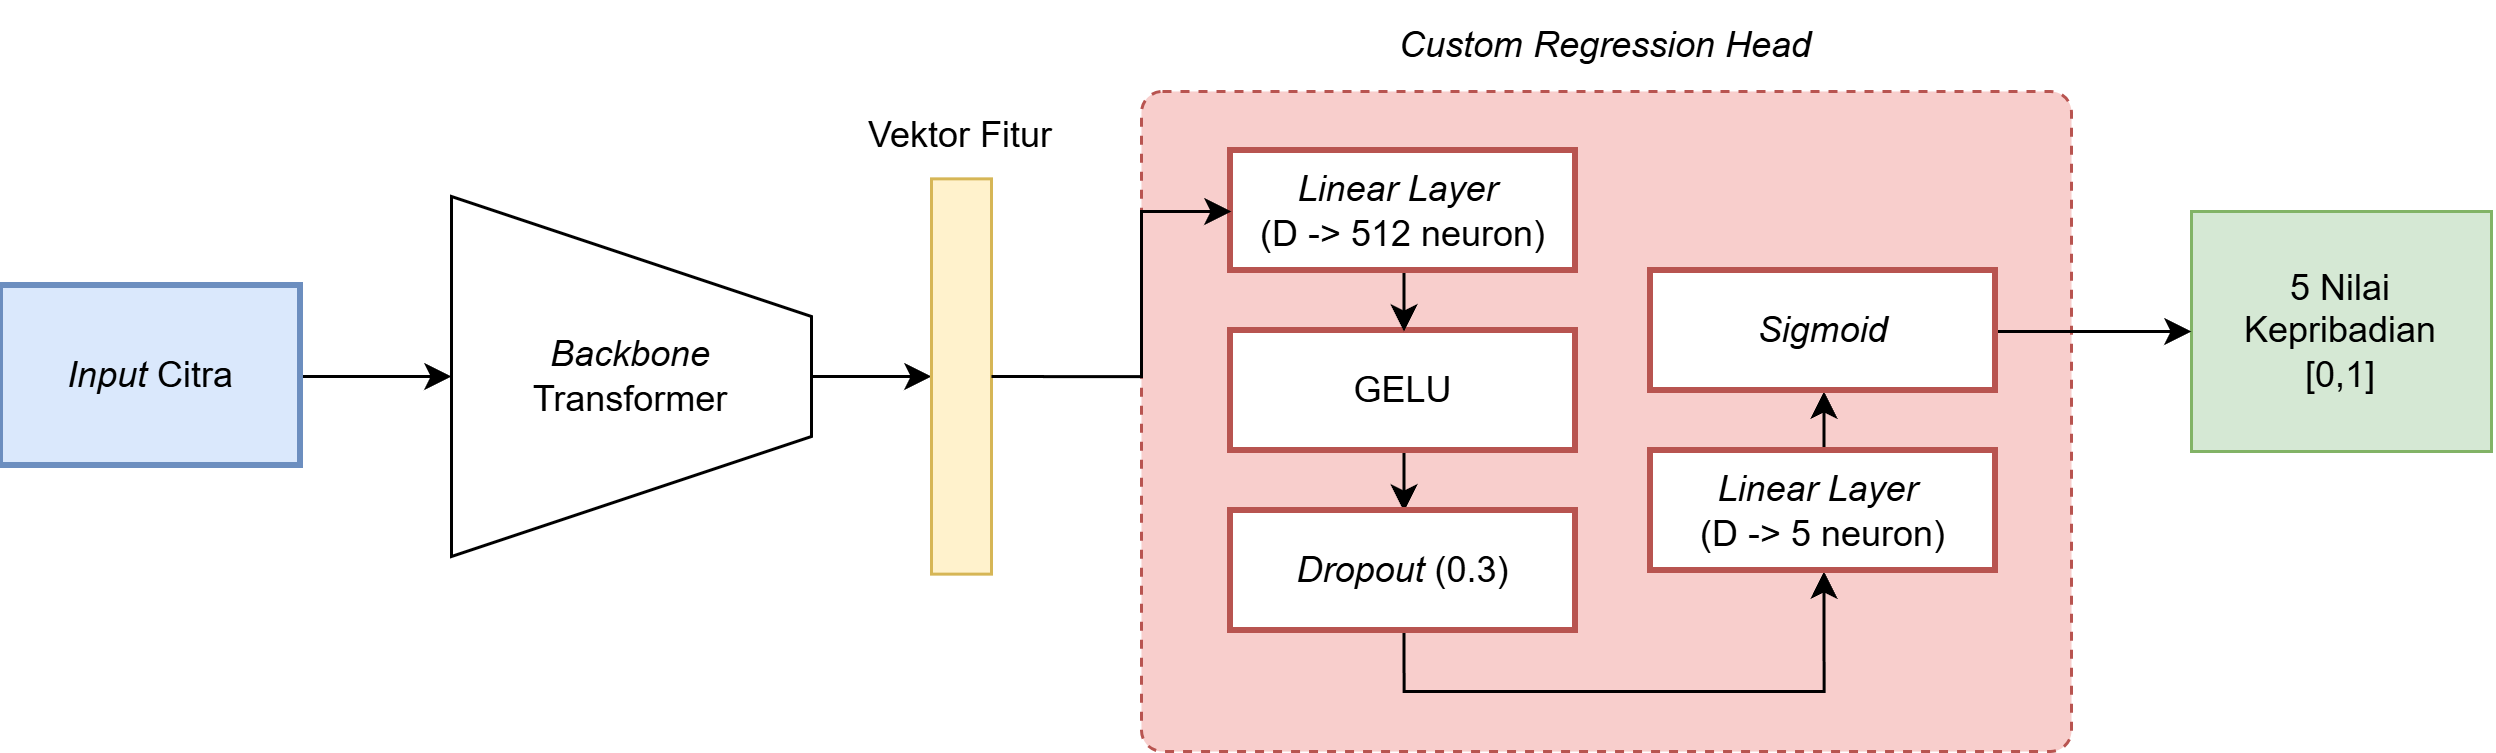
\includegraphics[width=\linewidth]{gambar/custom-transformer-arch-v2.png}
	\caption{Arsitektur Model Transformer untuk Regresi \textit{Multi Target}}
	\label{fig:custom-transformer-arch}
\end{figure}

\subsection{Mekanisme Prediksi dan Pelatihan Model Kepribadian \textit{Big Five}}

Fitur visual dari input gambar awalnya diekstraksi oleh \textit{backbone} Transformer. Selanjutnya, model memasuki tahap pelatihan model dengan melakukan prediksi nilai kepribadian yang dilanjutkan dengan \textit{backpropagation} untuk memperbarui bobot model. Alur mekanisme ini diilustrasikan pada Gambar \ref{fig:training-prediction}.

\begin{figure}[H]
	\centering
	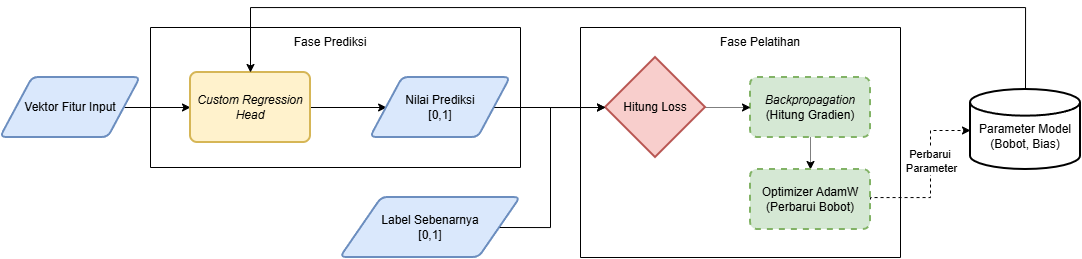
\includegraphics[width=\linewidth]{gambar/training-prediction.png}
	\caption{Proses Prediksi dan Pelatihan Model Prediksi Kepribadian \textit{Big Five}}
	\label{fig:training-prediction}
\end{figure}

Alur kerja model dibagi menjadi dua bagian, yaitu fase prediksi dan fase pelatihan untuk memperbarui bobot model.

\begin{enumerate}[nosep]

	\item Fase prediksi, vektor fitur yang yang dihasilkan oleh \textit{backbone} dipetakan menjadi lima nilai kepribadian. Proses ini dilakukan pada \textit{Custom Regression Head} yang dijelaskan pada subbab sebelumnya dengan label nilai kepribadian ChaLearn berada pada interval 0 hingga 1.

	\item Fase pelatihan, untuk memastikan model mampu menghasilkan prediksi yang akurat, dilakukan proses pelatihan yang bertujuan meminimalkan kesalahan prediksi. \textit{Loss function} yang digunakan adalah L1Loss atau MAE. MAE mengukur rata-rata absolut selisih antara nilai prediksi dan nilai label sebenarnya untuk kelima dimensi kepribadian \textit{Big Five}.
\end{enumerate}

Nilai \textit{loss} yang dihasilkan oleh MAE menjadi dasar bagi algoritma \textit{backpropagation} untuk menghitung gradien kesalahan terhadap parameter model. Berdasarkan gradien tersebut, \textit{optimizer} AdamW memperbarui bobot model secara iteratif. Penggunaan AdamW dipilih karena kemampuannya dalam menangani \textit{weight decay} yang lebih efektif dibandingkan Adam standar sehingga membantu mencegah \textit{overfitting} pada model berbasis Transformer.

\subsection{Perancangan \textit{Prompt} Interpretasi Kepribadian}
\label{subsec:rancangan-prompt}

\textit{Output} dari model regresi berupa lima nilai numerik \textit{Big Five}, misalnya \textit{Openness} 0.85 dan \textit{Neuroticism} 0.20 memberikan representasi kuantitatif namun sulit dipahami secara intuitif oleh pengguna awam. Oleh karena itu, diperlukan jembatan linguistik untuk menerjemahkan angka-angka tersebut menjadi narasi profil kepribadian yang deskriptif. Bagian ini membahas perancangan \textit{prompt} yang berfungsi memandu LLM dalam menyusun interpretasi tersebut. Perancangan \textit{prompt} dalam tugas akhir ini menerapkan dua strategi utama, yaitu \textit{role-play prompting} yang bertujuan menetapkan persona spesifik kepada LLM untuk memastikan \textit{tone} dan gaya bahasa yang dihasilkan bersifat profesional dan psikologis, serta penggunaan \textit{contextual injection} untuk menyematkan data hasil prediksi yang berupa skor numerik dan data visual, yaitu citra wajah secara dinamis ke dalam struktur \textit{prompt} sebagai konteks penalaran utama.

\begin{figure}[H]
	\centering
	\begin{tikzpicture}[scale=0.73, transform shape]
		% Style untuk Box Utama
		\node [draw=black!60, fill=white, thick, rectangle, rounded corners, inner sep=20pt, text width=19cm, align=left, drop shadow={opacity=0.3, shadow xshift=3pt, shadow yshift=-3pt}] (box){

			% --- BAGIAN 1: ROLE ---
			\textbf{\textcolor{blue!60!black}{[SYSTEM INSTRUCTION]}}\\
			\textit{Anda adalah seorang psikolog ahli dalam menganalisis kepribadian tampak. Berikan wawasan mendalam dengan cara yang empatik, ramah, konstruktif, seolah-olah Anda sedang memberikan konseling kepada pengguna, tetapi JANGAN sebutkan diri Anda sebagai psikolog kepada pengguna secara langsung."}\\
			\vspace{0.4cm}
			
			% --- BAGIAN 2: VISUAL ---
			\textbf{\textcolor{red!70!black}{[VISUAL CONTEXT]}}\\
			\texttt{<image\_token>} \\
			\vspace{0.4cm}
			
			% --- BAGIAN 3: DATA INJECTION ---
			\textbf{\textcolor{orange!80!black}{[NUMERICAL CONTEXT]}}\\
			Berdasarkan prediksi kepribadian Big Five berikut yang diekstraksi dari wajah pengguna:
			\begin{itemize}[nosep]
				\item Openness (Keterbukaan): \texttt{\{val\_O\}}
				\item Conscientiousness (Kehati-hatian): \texttt{\{val\_C\}}
				\item Extraversion (Ekstraversi): \texttt{\{val\_E\}}
				\item Agreeableness (Keramahan): \texttt{\{val\_A\}}
				\item Neuroticism (Neurotisisme): \texttt{\{val\_N\}}
			\end{itemize}
			\vspace{0.2cm}

			% --- BAGIAN 4: TASK ---
			\textbf{\textcolor{green!40!black}{[TASK INSTRUCTION]}}\\
			Berikan asesmen kepribadian yang mendetail dan komprehensif. Analisis fitur visual dari gambar yang mungkin berkorelasi dengan sifat-sifat psikologis ini. Fokus hanya kepada asesmen kepribadian. Gunakan bahasa indonesia yang baik dan benar. \\
			CATATAN : berikan respon maksimal 1500 token
		};

		%		% Judul di atas box
		%		\node[above=0.2cm of box, font=\bfseries\large] {Template Struktur Prompt Integrasi};

	\end{tikzpicture}
	\caption{Rancangan Struktur Prompt dengan Injeksi Konteks Multimodal}
	\label{fig:prompt-structure}
\end{figure}

Struktur prompt disusun secara sistematis menjadi empat segmen blok informasi yang diilustrasikan pada Gambar \ref{fig:prompt-structure}.

\begin{enumerate}[nosep]
	\item \textbf{\textit{System Instruction}}: Blok ini mendefinisikan peran LLM sebagai seorang ahli psikologi dan perilaku manusia. Instruksi ini bertujuan membatasi ruang pencarian model agar fokus pada terminologi psikologi kepribadian dan menghindari penggunaan bahasa yang terlalu teknis atau tidak relevan.
	
	\item \textbf{\textit{Visual Context}}: Blok ini menyertakan token khusus untuk memuat citra wajah subjek yang sudah diubah dalam bentuk Base64.

	\item \textbf{\textit{Numerical Context}}: Blok ini berisi variabel yang diisi dengan nilai prediksi dari model regresi. Format penyajian data dibuat terstruktur sebagai pasangan \textit{key-value} agar mudah dibaca oleh LLM.

	\item \textbf{\textit{Task Instruction}}: Bagian ini berisi perintah spesifik mengenai format \textit{output} yang diinginkan seperti batasan jumlah kata, penggunaan paragraf naratif, serta larangan untuk membuat asumsi di luar data yang diberikan.

\end{enumerate}

\subsection{Integrasi LLM untuk Interpretasi Kepribadian}

Tahap selanjutnya dari arsitektur sistem adalah interpretasi kepribadian menggunakan LLM. Pada tahap ini, sistem mengintegrasikan data prediksi nilai kepribadian \textit{Big Five} dengan inferensi LLM menggunakan layanan OpenRouter API. Alur integrasi sistem dirancang secara linear mulai dari akuisisi data, konstruksi \textit{payload}, hingga hasil interpretasi diilustrasikan pada Gambar \ref{fig:llm-integration}.

\begin{figure}[H]
	\centering
	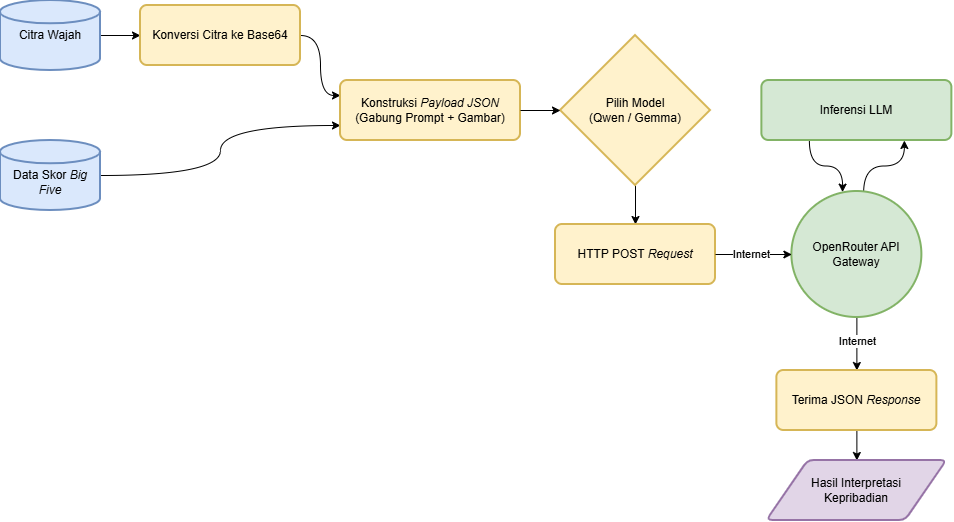
\includegraphics[width=\linewidth]{gambar/llm-integration.png}
	\caption{Diagram Alir Proses Interpretasi Kepribadian dengan LLM}
	\label{fig:llm-integration}
\end{figure}

Proses integrasi ini terdiri dari lima tahapan utama:

\begin{enumerate}[nosep]
	\item \textbf{Praproses Input}, sistem mengambil dua jenis data input, yaitu citra wajah dan data skor \textit{Big Five} yang merupakan nilai numerik hasil prediksi model regresi untuk dimasukkan ke dalam \textit{prompt}. Data citra dikonversi menjadi Base64 untuk mengubah data biner menjadi \textit{string} teks ASCII agar dapat ditransmisikan melalui protokol HTTP sebagai bagian dari objek JSON.

	\item \textbf{Konstruksi \textit{Payload}}, data citra yang berupa \textit{string} Base64 dan skor \textit{Big Five} digabungkan dan disusun ke dalam \textit{message structure} yang berisi instruksi sistem dan konteks visual.

	\item \textbf{Pemilihan Model}, disediakan dua model LLM untuk inferensi, yaitu Gemma 4 dan Qwen3-VL. Pemilihan ini menentukan parameter ID model yang akan dikirimkan ke server.

	\item \textbf{\textit{API Reguest}}, setelah \textit{payload} siap, sistem mengirimkan HTTP POST \textit{Request} melalui jaringan internet menuju OpenRouter API Gateway. Di sisi server, permintaan diteruskan ke mesin Inferensi LLM sesuai model yang dipilih untuk diproses.

	\item \textbf{Penyajian Hasil}, setelah proses inferensi selesai, sistem akan menerima JSON \textit{Response} dari server. Respons ini kemudian dilakukan \textit{parsing} untuk diambil konten teks utama yang kemudian ditampilkan sebagai hasil interpretasi kepribadian.
\end{enumerate}

\subsection{Perancangan Sistem Asesmen Interpretasi Kepribadian}

Sistem asesmen interpretasi kepribadian disusun sebagai sarana untuk mengakses model prediksi dan interpretasi kepribadian secara terintegrasi menggunakan \textit{Application Programming Interface} (API). Tujuan dari penggunaan API adalah untuk memudahkan pengguna mengakses dan menggunakan sistem. Mekanisme komunikasi pada sistem ditunjukkan oleh gambar \ref{fig:assesment-system}.

\begin{figure}[H]
	\centering
	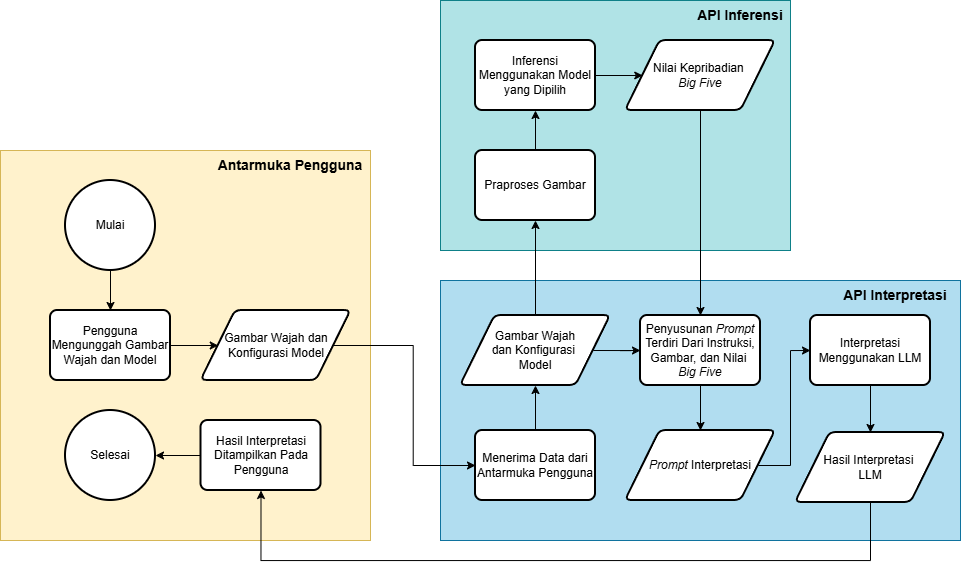
\includegraphics[width=0.9\linewidth]{gambar/assesment-system.png}
	\caption{Diagram Alir Sistem Interpretasi Kepribadian}
	\label{fig:assesment-system}
\end{figure}

Sistem ini terdiri dari tiga komponen, yaitu API Inferensi, API Interpretasi, dan antarmuka pengguna. 

\subsubsection{API Inferensi}
API inferensi menyediakan akses bagi pengguna untuk melakukan prediksi nilai kepribadian \textit{Big Five}. Tugas dari API inferensi meliputi praproses gambar yang diterima dari pengguna dan inferensi menggunakan model prediksi. Komponen ini menghasilkan nilai kepribadian \textit{Big Five} yang akan digunakan pada tahap interpretasi selanjutnya. 

\subsubsection{API Interpretasi}
API interpretasi merupakan sistem yang mengintegrasikan API inferensi dengan layanan OpenRouter API untuk menghasilkan deskripsi interpretasi kepribadian yang dapat dipahami oleh pengguna. API interpretasi memiliki beberapa tugas untuk menghasilkan hasil interpretasi kepribadian dari input berupa gambar yang dikirim oleh pengguna, yaitu:

\begin{enumerate}[nosep]
	\item Menerima \textit{request} dari pengguna untuk melakukan interpretasi berdasarkan konfigurasi yang diberikan.
	\item Mengirim gambar dan konfigurasi model ke API inferensi untuk mendapatkan hasil prediksi kepribadian \textit{Big Five}.
	\item Melakukan konversi gambar menjadi \textit{string} Base64 agar dapat dipahami oleh LLM, menyusun \textit{prompt} yang meliputi instruksi sistem, token gambar Base64, hasil prediksi kepribadian \textit{Big Five}, serta instruksi tugas untuk menghasilkan interpretasi kepribadian pengguna.
	\item Mengirimkan \textit{request prompt} ke LLM melalui OpenRouter API dan menerima respons hasil.
	\item Mengirimkan hasil interpretasi kepribadian kepada pengguna.    
\end{enumerate}

\subsubsection{Antarmuka Pengguna}

Untuk menjembatani interaksi antara pengguna dengan sistem, diperlukan tampilan antarmuka grafis yang dapat diakses dengan mudah dan intuitif. Antarmuka ini dirancang untuk menguji sistem inferensi dan interpretasi kepribadian menggunakan aplikasi berbasis web. Tahap pertama yang dilakukan adalah proses \textit{wireframing}, yaitu perancangan kerangka \textit{website} yang meliputi struktur dan tata letak komponen dasar. Terdapat dua tampilan antarmuka yang disusun, yaitu tampilan inferensi yang digunakan untuk menguji sistem API Inferensi dan tampilan interpretasi yang digunakan untuk menguji sistem API Interpretasi.

\begin{figure}[H]
	\centering
	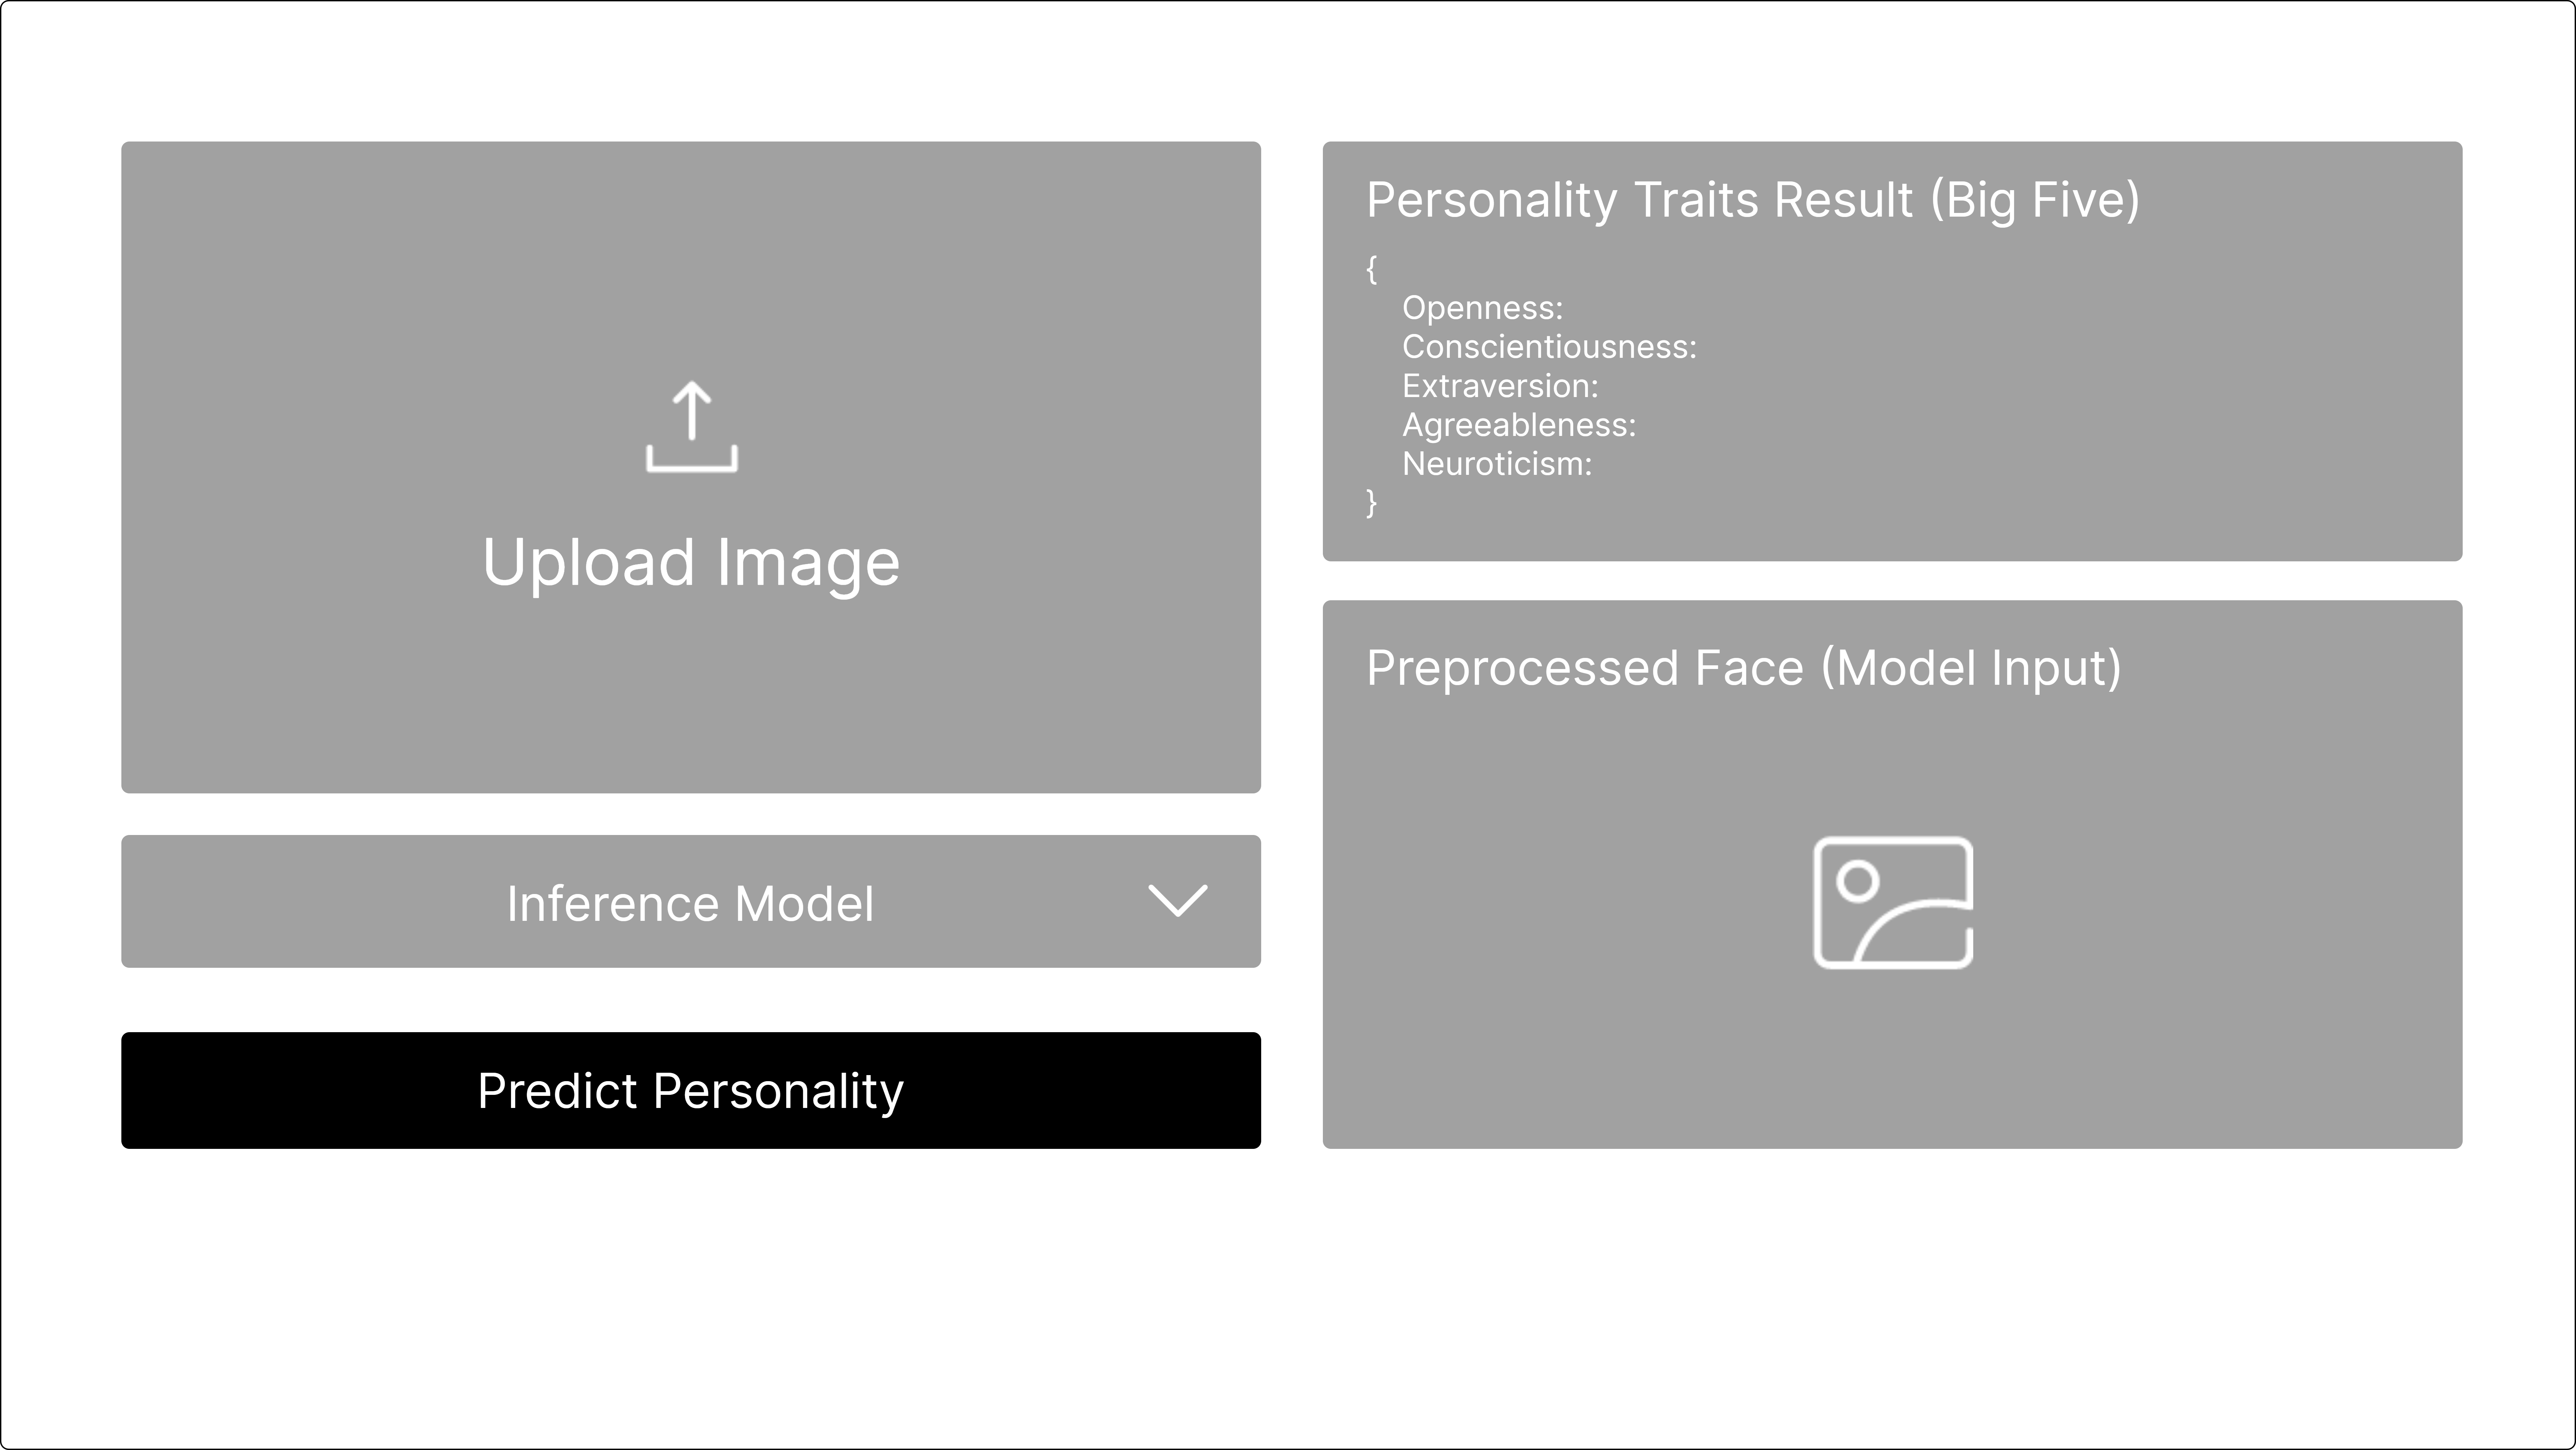
\includegraphics[width=0.9\linewidth]{gambar/inference-interface.png}
	\caption{\textit{Wireframe} Tampilan Inferensi}
	\label{fig:antarmuka-inferensi}
\end{figure}

Alur pengggunaan antarmuka inferensi dimulai dari pengguna mengunggah gambar wajah pada bagian \textit{upload image} dan memilih model inferensi yang diinginkan pada bagian \textit{inference model}. Pengguna kemudian menekan tombol \textit{predict personality} untuk mengirim \textit{request} menuju server. Hasil yang didapatkan berupa nilai kepribadian \textit{Big Five} dan gambar hasil praproses yang digunakan model prediksi kepribadian untuk melakukan inferensi. Prototipe tampilan antarmuka inferensi dapat dilihat pada Gambar \ref{fig:antarmuka-inferensi}.

Selanjutnya untuk antarmuka interpretasi digunakan untuk menguji integrasi antara API Interpretasi, API Inferensi, dan layanan LLM melalui OpenRouter API. Prototipe tampilan antarmuka interpretasi ditunjukkan oleh Gambar \ref{fig:antarmuka-interpretasi}. Pengguna mengunggah gambar wajah, kemudian memilih model inferensi yang tersedia pada API Inferensi, selanjutnya pengguna memilih LLM dan gaya respons yang digunakan. \textit{Output} yang dihasilkan setelah pengguna menekan tombol \textit{interpret personality} adalah hasil prediksi \textit{Big Five} dan deskripsi interpretasi kepribadian yang dihasilkan dari LLM. Pengguna juga dapat menyimpan hasil interpretasi dalam bentuk JSON yang dapat digunakan untuk evaluasi hasil interpretasi kepribadian.  

\begin{figure}[H]
	\centering
	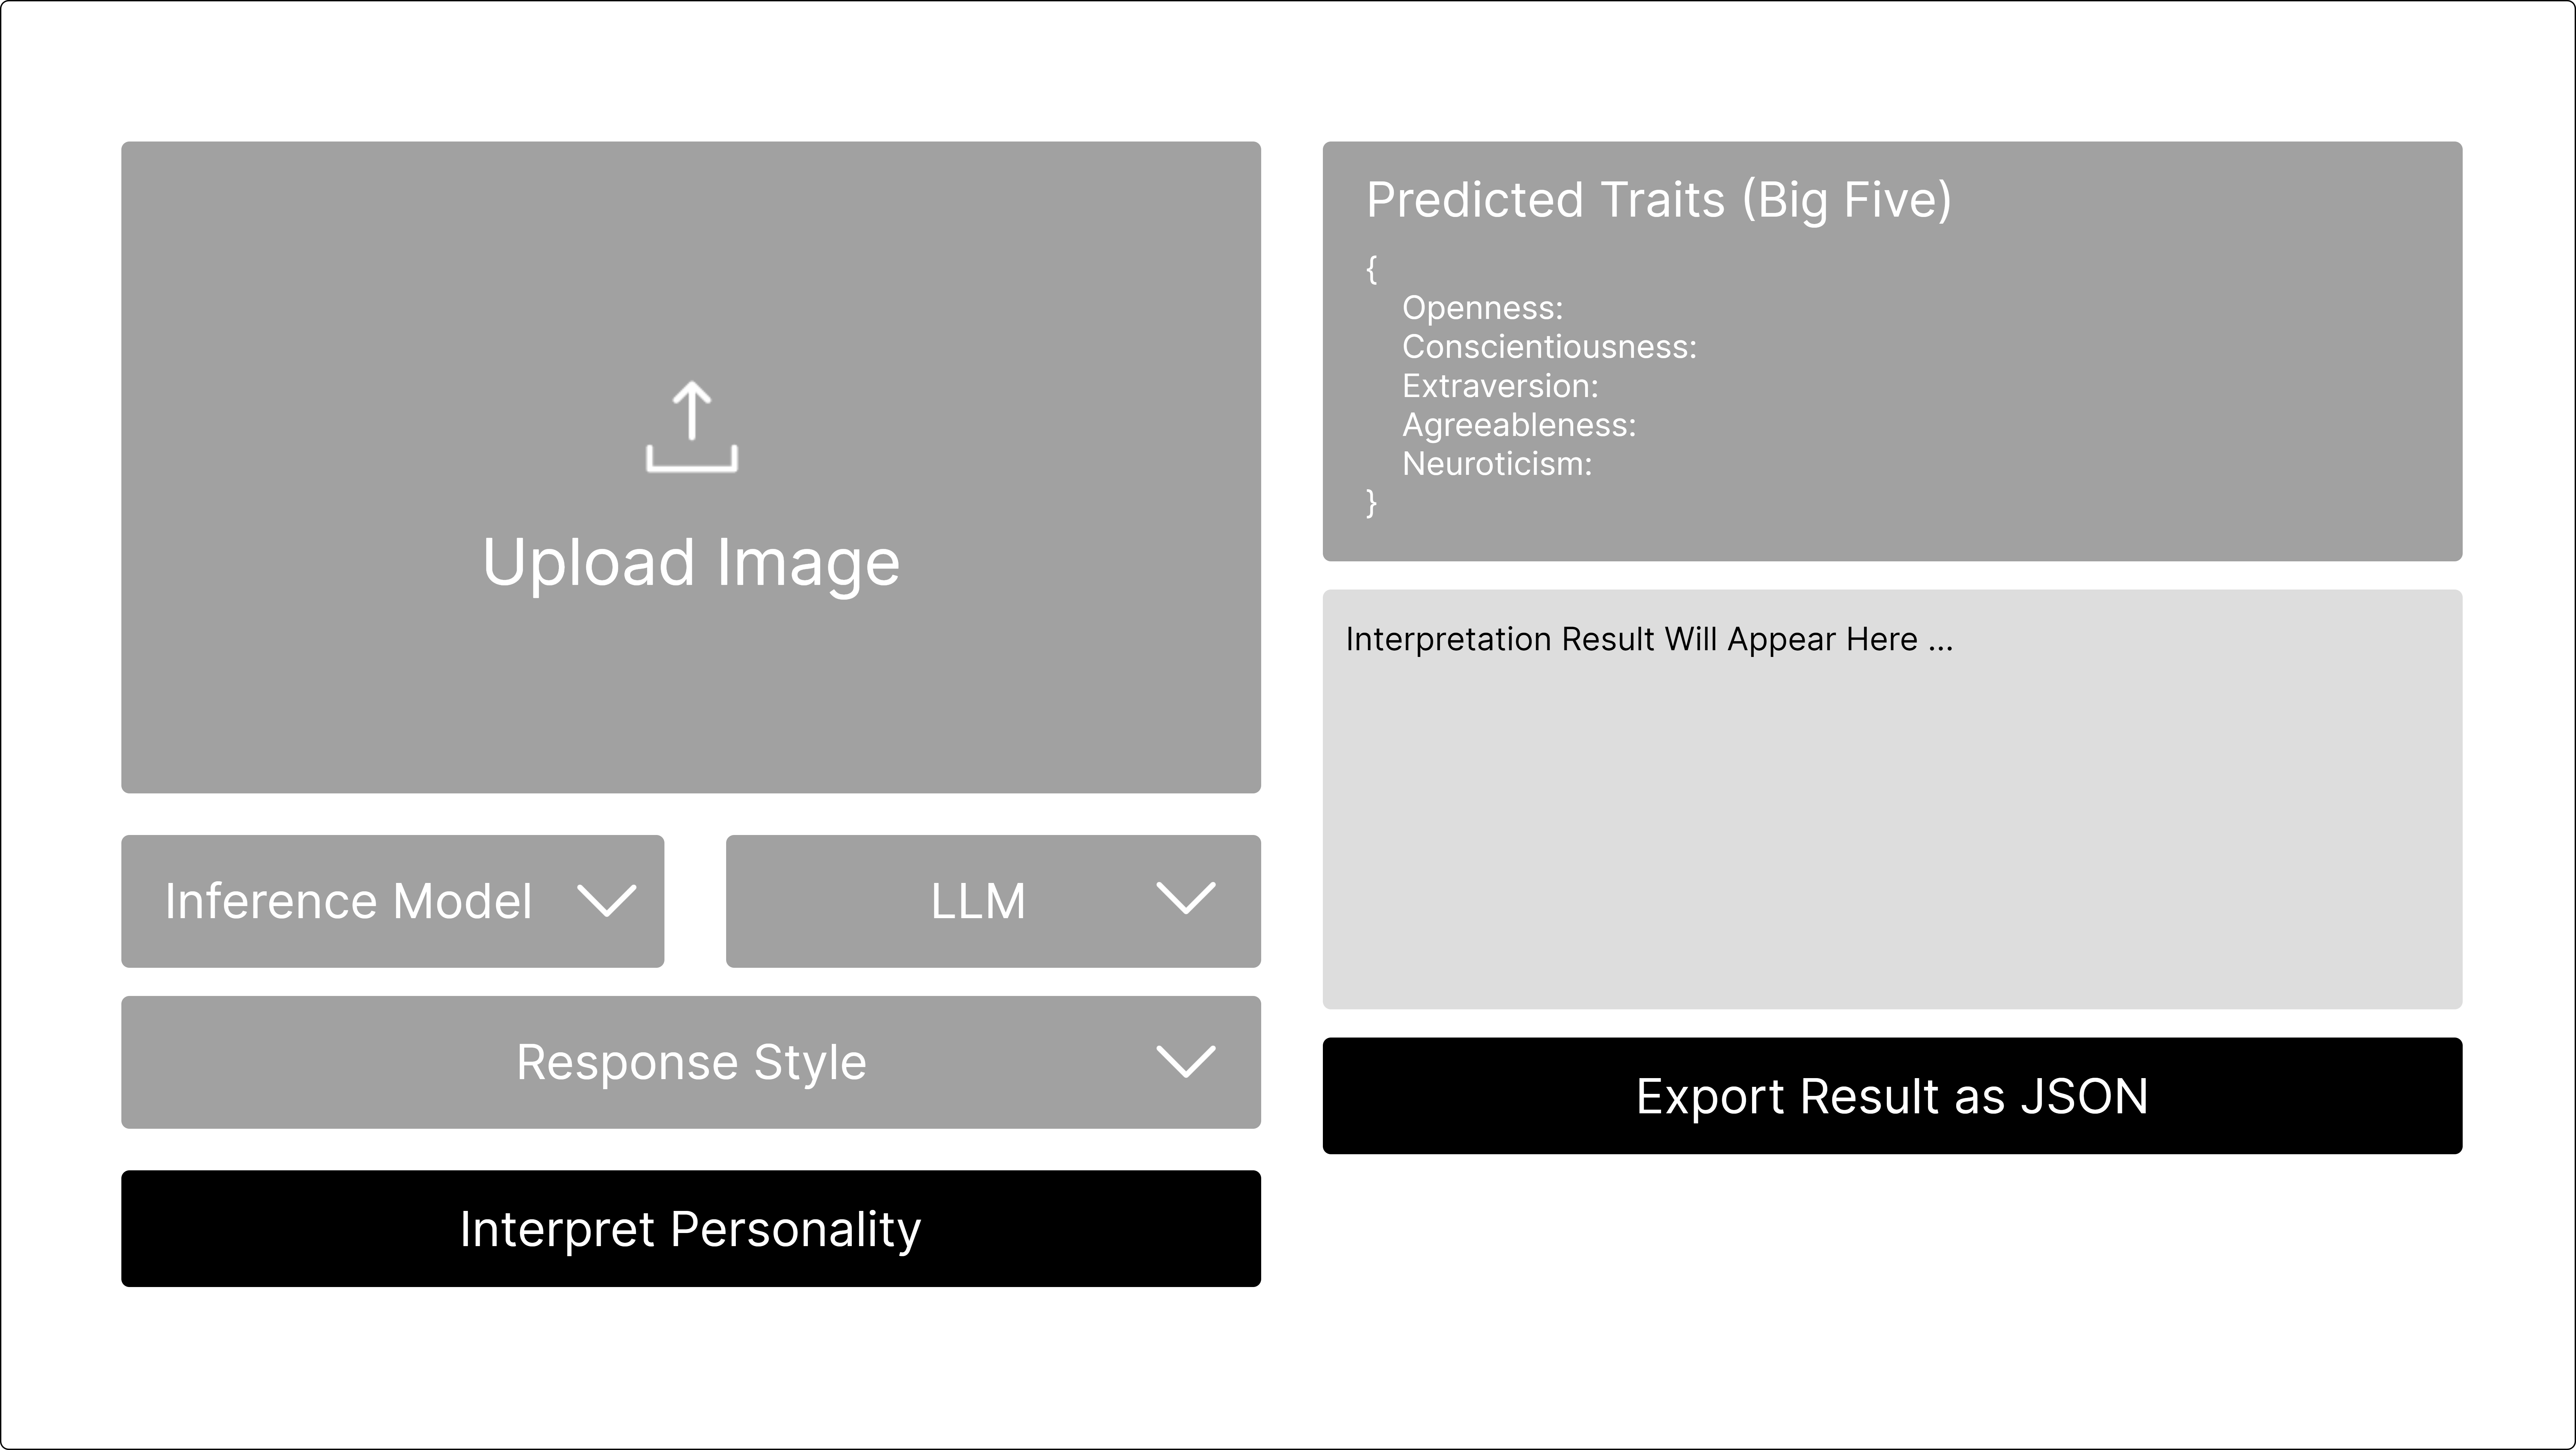
\includegraphics[width=0.9\linewidth]{gambar/interpretation-interface.png}
	\caption{\textit{Wireframe} Tampilan Interpretasi}
	\label{fig:antarmuka-interpretasi}
\end{figure}

\subsection{Skenario Evaluasi}

Evaluasi terhadap sistem asesmen kepribadian ini dilakukan secara komprehensif yang terbagi dalam dua fokus pengujian utama. Aspek pertama ditujukan untuk mengukur tingkat akurasi kinerja model regresi dalam memprediksi nilai numerik kepribadian \textit{Big Five}. Selanjutnya, aspek kedua difokuskan untuk mengevaluasi kualitas dan kelayakan teks interpretasi deskriptif kepribadian yang dihasilkan oleh LLM.

\subsubsection{Evaluasi Model Prediksi Kepribadian \textit{Big Five}}

Evaluasi model prediksi dilakukan dengan mengukur akurasi prediksi nilai numerik kepribadian terhadap nilai ground truth. Tugas akhir ini menggunakan metrik evaluasi regresi standar yang meliputi MAE untuk mengukur rata-rata kesalahan absolut prediksi, $\text{Accuracy}$ untuk merepresentasikan tingkat ketepatan model dalam skala 0 hingga 1, RMSE untuk mendeteksi kesalahan prediksi yang bernilai besar, serta \textit{Coefficient of Determination} ($R^2$) untuk melihat seberapa baik model dapat menjelaskan variabilitas data. Metrik utama yang digunakan untuk menentukan model terbaik adalah $\text{Accuracy}$ Terdapat 6 model \textit{pretrained} yang diujikan. Model-model yang diujikan ditunjukkan oleh \autoref{tab:model-list}.

{
	\footnotesize
	\renewcommand{\arraystretch}{1.3} % Melonggarkan spasi antar baris
	\noindent
	
	% Memulai xltabular dengan mengatur lebarnya menjadi \textwidth
	% c = rata tengah (pas dengan isi), l = rata kiri (pas dengan isi), X = rata kiri (mengisi sisa ruang)
	\begin{xltabular}{\textwidth}{|
			>{\hsize=0.7\hsize}X |
			>{\hsize=1.3\hsize}X | }
		
		% --- Caption diletakkan di dalam lingkungan xltabular ---
		\caption{Daftar Model Transformer \textit{Pretrained} yang Diujikan} 
		\label{tab:model-list} \\
		
		% --- Header Halaman Pertama ---
		\hline
		\centering\textbf{Model} & \centering\textbf{Deskripsi} \arraybackslash \\ \hline
		\endfirsthead
		
		% --- Header Halaman Lanjutan (Jika Terpotong ke Halaman Berikutnya) ---
		\caption*{Lanjutan \autoref{tab:model-list}} \\
		\hline
		\centering\textbf{Model} & \textbf{Deskripsi} \arraybackslash \\ \hline
		\endhead
		
		% --- Footer Sementara (Muncul di bawah halaman jika tabel terpotong) ---
		\hline
		\multicolumn{2}{r}{\textit{Berlanjut ke halaman berikutnya...}} \\
		\endfoot
		
		% --- Footer Paling Akhir (Muncul di akhir tabel) ---
		\hline
		\endlastfoot
		
		% --- Isi Data Tabel ---
		ViT-B/16 AugReg (IN21k) &  Model \textit{backbone} klasifikasi ViT yang dilatih dengan dataset ImageNet-21k dengan tambahan augmentasi dan regularisasi. \\ \hline
		ViT-B/16 AugReg (IN21k+1k) & Model \textit{backbone} klasifikasi ViT yang dilatih dengan dataset ImageNet-21k dan dilakukan \textit{fine-tuning} pada ImageNet-1k dengan tambahan augmentasi dan regularisasi. \\ \hline
		ViT-B/16 AugReg2 (IN21k+1k) & Model \textit{backbone} klasifikasi ViT yang dilatih dengan dataset ImageNet-21k dan dilakukan \textit{fine-tuning} ulang pada ImageNet-1k dengan tambahan augmentasi yang lebih kompleks dan regularisasi. \\ \hline
		SwinV2-B w16 (IN1k) & Model \textit{backbone} klasifikasi Swin Transformer v2 dengan ukuran \textit{window} $16 \times 16$ yang dilatih dengan dataset ImageNet-1k.  \\ \hline
		SwinV2-B w12-16 (IN22k+1k) & Model \textit{backbone} klasifikasi Swin Transformer v2 dengan ukuran \textit{window} $12 \times 12$ yang dapat diperbesar menjadi $16 \times 16$, dilatih dengan dataset ImageNet-22k dan dilakukan \textit{fine-tuning} menggunakan dataset ImageNet-1k. \\ \hline
		PVTv2-B5 (IN1k) & Model \textit{backbone} klasifikasi PVT-v2 yang dilatih dengan dataset ImageNet-1k. \\ \hline
		% Anda bisa menyalin dan menambahkan puluhan baris data lagi ke bawah sini
		
	\end{xltabular}
}

Setiap model dilatih menggunakan \textit{hyperparameter} yang dijelaskan pada \autoref{tab:hyperparameter}. Proses pelatihan menggunakan \textit{early stopping} dengan $\text{\textit{patience}} = 5$ untuk mencegah \textit{overfitting}. Pelatihan model menggunakan strategi \textit{differential learning rate} dimana bagian \textit{backbone} dilatih dengan \textit{learning rate} yang lebih kecil dari \textit{regression head} untuk melindungi generalisasi fitur yang telah dipelajari pada \textit{backbone} model \textit{pretrained} dan mempercepat konvergensi pada \textit{regression head}. \textit{Learning rate} pada pelatihan model untuk setiap \textit{epoch} disesuaikan secara dinamis menggunakan \textit{cosine annealing scheduler}, dimana \textit{learning rate} diturunkan secara bertahap mengikuti kurva kosinus hingga maksimal parameter yang ditentukan. Hal ini dilakukan agar model dapat mencapai titik konvergensi yang lebih presisi. Penurunan nilai \textit{learning rate} yang semakin melandai di akhir proses pelatihan memungkinkan \textit{weight update} yang lebih halus sehingga mencegah model mengalami osilasi saat sudah berada di dekat titik minimum \textit{loss} global. Teknik \textit{gradient clipping} juga digunakan dengan \textit{L2Norm} untuk mencegah gradien yang terlalu besar (\textit{exploding gradient}) yang menyebabkan perubahan \textit{weight} secara drastis.

{
	\footnotesize
	\renewcommand{\arraystretch}{1.3} % Melonggarkan spasi antar baris
	
	% Menggunakan longtable biasa: lebar tabel akan pas dengan isi dan otomatis di tengah halaman
	% Kolom 1 (l) = rata kiri untuk nama hyperparameter
	% Kolom 2 (c) = rata tengah untuk nilainya
	\begin{longtable}{| l | c |}
		
		% --- Caption diletakkan di dalam lingkungan longtable ---
		\caption{Konfigurasi \textit{Hyperparameter} Pelatihan Model Prediksi Kepribadian} 
		\label{tab:hyperparameter} \\
		
		% --- Header Halaman Pertama ---
		\hline
		\centering\textbf{\textit{Hyperparameter}} & \textbf{Nilai} \\ \hline
		\endfirsthead
		
		% --- Header Halaman Lanjutan (Jika Terpotong ke Halaman Berikutnya) ---
		\caption*{Lanjutan \autoref{tab:hyperparameter}} \\
		\hline
		\centering\textbf{\textit{Hyperparameter}} & \textbf{Nilai} \\ \hline
		\endhead
		
		% --- Footer Sementara (Muncul di bawah halaman jika tabel terpotong) ---
		\hline
		\multicolumn{2}{r}{\textit{Berlanjut ke halaman berikutnya...}} \\
		\endfoot
		
		% --- Footer Paling Akhir (Muncul di akhir tabel) ---
		\hline
		\endlastfoot
		
		% --- Isi Data Tabel ---
		\textit{Batch Size} & 32  \\ \hline
		\textit{Epochs} & 100 \\ \hline
		\textit{Early Stopping Patience} & 5 \\ \hline
		\textit{Loss Function} & L1Loss (MAE) \\ \hline
		\textit{Gradient Clipping} & 1,0 (L2 Norm) \\ \hline
		\textit{Regression Head Learning Rate} & $1 \times 10^{-4}$ \\ \hline
		\textit{Backbone Learning Rate} & $1 \times 10^{-5}$ \\ \hline
		\textit{Weight Decay} & 0,01 \\ \hline
		\textit{Learning Rate Scheduler} & Cosine Annealing \\ \hline
		\textit{Minimum Learning Rate Scheduler} &  $1 \times 10^{-6}$ \\ \hline	
		
	\end{longtable}
}

%{
%	\renewcommand{\arraystretch}{1.3} % Melonggarkan spasi antar baris
%	\noindent
%	
%	% Memulai xltabular dengan mengatur lebarnya menjadi \textwidth
%	% c = rata tengah (pas dengan isi), l = rata kiri (pas dengan isi), X = rata kiri (mengisi sisa ruang)
%	\begin{xltabular}{\textwidth}{|
%			>{\hsize=0.7\hsize}X |
%			>{\hsize=1.3\hsize}X | }
%		
%		% --- Caption diletakkan di dalam lingkungan xltabular ---
%		\caption{Konfigurasi \textit{Hyperparameter} Pelatihan Model Prediksi Kepribadian} 
%		\label{tab:hyperparameter} \\
%		
%		% --- Header Halaman Pertama ---
%		\hline
%		\centering\textbf{\textit{Hyperparameter}} & \centering\textbf{Nilai} \arraybackslash \\ \hline
%		\endfirsthead
%		
%		% --- Header Halaman Lanjutan (Jika Terpotong ke Halaman Berikutnya) ---
%		\caption*{Lanjutan \autoref{tab:hyperparameter}} \\
%		\hline
%		\centering\textbf{\textit{Hyperparameter}} & \centering\textbf{Nilai} \arraybackslash \\ \hline
%		\endhead
%		
%		% --- Footer Sementara (Muncul di bawah halaman jika tabel terpotong) ---
%		\hline
%		\multicolumn{2}{r}{\textit{Berlanjut ke halaman berikutnya...}} \\
%		\endfoot
%		
%		% --- Footer Paling Akhir (Muncul di akhir tabel) ---
%		\hline
%		\endlastfoot
%		
%		% --- Isi Data Tabel ---
%		\textit{Batch Size} & 32  \\ \hline
%		\textit{Epochs} & 100 \\ \hline
%		\textit{Early Stopping Patience} & 5 \\ \hline
%		\textit{Loss Function} & L1Loss (MAE) \\ \hline
%		\textit{Gradient Clipping} & 1,0 (L2 Norm) \\ \hline
%		\textit{Regression Head Learning Rate} & $1 \times 10^{-4}$ \\ \hline
%		\textit{Backbone Learning Rate} & $1 \times 10^{-5}$ \\ \hline
%		\textit{Weight Decay} & 0,01 \\ \hline
%		\textit{Learning Rate Scheduler} & Cosine Annealing \\ \hline
%		\textit{Minimum Learning Rate Scheduler} &  $1 \times 10^{-6}$ \\ \hline	
%		% Anda bisa menyalin dan menambahkan puluhan baris data lagi ke bawah sini
%		
%	\end{xltabular}
%}

Selain itu, dilakukan uji ablasi dengan 4 jenis skenario yang dibuat untuk setiap model. Tujuan dari uji ablasi ini adalah untuk mengetahui pengaruh skenario yang diujikan terhadap kinerja model. Detail mengenai skenario yang diujikan dapat dilihat pada \autoref{tab:skenario-uji}.  

{
	\footnotesize
	\renewcommand{\arraystretch}{1.3} % Melonggarkan spasi antar baris
	\noindent
	
	% Memulai xltabular dengan mengatur lebarnya menjadi \textwidth
	% c = rata tengah (pas dengan isi), l = rata kiri (pas dengan isi), X = rata kiri (mengisi sisa ruang)
	\begin{xltabular}{\textwidth}{|c|
			>{\hsize=0.7\hsize}X |
			>{\hsize=1.3\hsize}X | }
		
		% --- Caption diletakkan di dalam lingkungan xltabular ---
		\caption{Daftar Skenario Model Prediksi yang Diujikan} 
		\label{tab:skenario-uji} \\
		
		% --- Header Halaman Pertama ---
		\hline
		\centering\textbf{No} & \centering\textbf{Skenario} & \centering\textbf{Penjelasan} \arraybackslash \\ \hline
		\endfirsthead
		
		% --- Header Halaman Lanjutan (Jika Terpotong ke Halaman Berikutnya) ---
		\caption*{Lanjutan \autoref{tab:skenario-uji}} \\
		\hline
		\centering\textbf{No} & \centering\textbf{Skenario} & \centering\textbf{Penjelasan} \arraybackslash \\ \hline
		\endhead
		
		% --- Footer Sementara (Muncul di bawah halaman jika tabel terpotong) ---
		\hline
		\multicolumn{3}{r}{\textit{Berlanjut ke halaman berikutnya...}} \\
		\endfoot
		
		% --- Footer Paling Akhir (Muncul di akhir tabel) ---
		\hline
		\endlastfoot
		
		% --- Isi Data Tabel ---
		1 & \textit{Baseline} & Skenario ini menggunakan model \textit{pretrained} dengan adaptasi \textit{regression head} menggunakan \textit{linear layer} dengan 5 neuron dan \textit{hidden layer} sigmoid sebagai pembanding dasar model prediksi untuk 5 sifat kepribadian \textit{Big Five} tanpa augmentasi gambar pada tahap praproses dataset latih. \\ \hline
		2 & \textit{Arch Tuning} & Skenario ini menggunakan model \textit{pretrained} dengan \textit{custom regression head} yang dijelaskan pada \autoref{subsec:arsitektur-regresi-bigfive} tanpa augmentasi gambar pada tahap praproses dataset latih. \\ \hline
		3 & Augmentasi & Skenario ini menggunakan model \textit{pretrained} yang sama seperti skenario \textit{baseline}, dengan menggunakan proses augmentasi gambar pada tahap praproses dataset latih seperti yang dijelaskan pada \autoref{subsec:praproses-dataset}. \\ \hline
		4 & \textit{Arch Tuning} + Augmentasi & Skenario ini merupakan gabungan dari skenario 2 dan 3 yang menggunakan model \textit{pretrained} dengan \textit{custom regression head} yang dijelaskan pada \autoref{subsec:arsitektur-regresi-bigfive} dan menggunakan alur praproses dataset yang dijelaskan pada \autoref{subsec:praproses-dataset}. \\ \hline
		% Anda bisa menyalin dan menambahkan puluhan baris data lagi ke bawah sini
		
	\end{xltabular}
}

\subsubsection{Evaluasi Kualitas Interpretasi Kepribadian}

Evaluasi kualitas teks interpretasi dilakukan menggunakan G-Eval dengan GPT-5.1 sebagai evaluator. Pendekatan ini dipilih karena GPT-5.1 memiliki korelasi tinggi dengan penilaian manusia dan mampu melakukan penalaran bertahap (\textit{Chain-of-Thought}) dalam memberikan skor. Terdapat tiga jenis kriteria yang digunakan dalam mengevaluasi teks hasil generasi interpretasi kepribadian yang ditunjukkan oleh \autoref{tab:kriteria-eval-llm}. Tiga kriteria ini ditujukan untuk menilai kualitas hasil generasi teks layaknya seorang psikolog profesional yang melakukan asesmen kepribadian sesuai dengan gambar yang diberikan. G-Eval memberikan nilai antara 0 hingga 1 untuk setiap kriteria yang diberikan. Terdapat dua jenis skenario yang dibuat untuk menguji pengaruh \textit{role-play prompt} terhadap kualitas narasi interpretasi kepribadian yang dihasilkan. Skenario 1 adalah skenario menggunakan rancangan \textit{prompt} yang dijelaskan pada \autoref{subsec:rancangan-prompt} dan skenario 2 adalah skenario 1 tanpa menggunakan strategi \textit{role-play prompting} sehingga \textit{prompt} yang disusun terdiri dari tiga segmen blok informasi tanpa \textit{System Instruction}.

{
	\footnotesize
	\renewcommand{\arraystretch}{1.3} % Melonggarkan spasi antar baris
	\noindent
	
	% Memulai xltabular dengan mengatur lebarnya menjadi \textwidth
	% c = rata tengah (pas dengan isi), l = rata kiri (pas dengan isi), X = rata kiri (mengisi sisa ruang)
	\begin{xltabular}{\textwidth}{|c|
			>{\hsize=0.5\hsize}X |
			>{\hsize=1.5\hsize}X | }
		
		% --- Caption diletakkan di dalam lingkungan xltabular ---
		\caption{Kriteria Evaluasi Teks Interpretasi Kepribadian dengan G-Eval} 
		\label{tab:kriteria-eval-llm} \\
		
		% --- Header Halaman Pertama ---
		\hline
		\centering\textbf{No} & \centering\textbf{Jenis Kriteria} & \centering\textbf{Deskripsi} \arraybackslash \\ \hline
		\endfirsthead
		
		% --- Header Halaman Lanjutan (Jika Terpotong ke Halaman Berikutnya) ---
		\caption*{Lanjutan \autoref{tab:kriteria-eval-llm}} \\
		\hline
		\centering\textbf{No} & \centering\textbf{Jenis Kriteria} & \centering\textbf{Deskripsi} \arraybackslash \\ \hline
		\endhead
		
		% --- Footer Sementara (Muncul di bawah halaman jika tabel terpotong) ---
		\hline
		\multicolumn{3}{r}{\textit{Berlanjut ke halaman berikutnya...}} \\
		\endfoot
		
		% --- Footer Paling Akhir (Muncul di akhir tabel) ---
		\hline
		\endlastfoot
		
		% --- Isi Data Tabel ---
		1 & Koherensi Gambar & Menilai kesesuaian dan konsistensi fitur fisik atau kesan visual dalam teks interpretasi kepribadian dengan gambar yang diberikan. \\ \hline
		2 & Akurasi Penilaian Psikologis & Mengevaluasi akurasi dan kesesuaian interpretasi kepribadian terhadap nilai kepribadian \textit{Big Five} yang diberikan. \textit{Openness} tinggi harus berkaitan dengan deskripsi kreativitas/rasa ingin tahu. \textit{Conscientiousness} tinggi harus menyebutkan kedisiplinan/keteraturan. Extraversion tinggi harus menggambarkan keramahan sosial. \textit{Agreeableness} tinggi harus merujuk pada kerja sama/empati. \textit{Neuroticism} tinggi harus sesuai dengan sensitivitas emosional. Skor rendah jika teks bertentangan atau mengabaikan skor kepribadian.\\ \hline
		3 & Persona Psikolog & Mengevaluasi persona/gaya teks generasi interpretasi kepribadian layaknya seorang psikolog yang memberikan asesmen kepribadian dengan nada empatik, hangat, dan profesional yang terwujud secara natural tanpa menyebutkan diri sebagai seorang psikolog. Skor rendah jika kesan respons terlalu kaku, dingin, atau santai. \\
		
		% Anda bisa menyalin dan menambahkan puluhan baris data lagi ke bawah sini
		
	\end{xltabular}
}

\section{Bahan dan Peralatan yang Digunakan}

Tugas akhir ini dilaksanakan menggunakan peralatan pendukung yang terdiri dari perangkat keras dan perangkat lunak. Perangkat keras yang digunakan adalah laptop HP Victus 15 dengan prosesor AMD Ryzen 5 240, RAM 16GB, dan GPU NVIDIA RTX 5050 yang digunakan untuk pengembangan kode dan praproses data, serta sumber daya \textit{cloud computing} menggunakan platform runpod yang menyediakan GPU NVIDIA RTX 5090 dengan VRAM 32GB untuk akselerasi proses pelatihan model. Selain itu, Huggingface Spaces dan Azure VM digunakan untuk proses \textit{deployment} sistem asesmen kepribadian yang meliputi tahap inferensi dan interpretasi. Adapun perangkat lunak yang digunakan adalah Jupyter Notebook yang menyediakan lingkungan pelatihan model. Implementasi sistem dibangun menggunakan bahasa pemrograman Python dengan dukungan \textit{library} PyTorch Image Models (timm) untuk \textit{deep learning}, MediaPipe dan OpenCV untuk pengolahan visual, serta penggunaan OpenRouter API untuk mengakses LLM yang digunakan dalam tahap interpretasi.

\section{Urutan Pelaksanaan Penelitian}

Bagian ini menguraikan secara rinci langkah-langkah teknis dan urutan pelaksanaan yang dilakukan selama penelitian ini berlangsung. Rangkaian tahapan tersebut mencakup implementasi praproses dataset visual, alur pelatihan model prediksi regresi, perancangan sistem asesmen kepribadian, hingga proses evaluasi kinerja akhir. Guna memberikan pemahaman yang komprehensif mengenai logika komputasi yang diterapkan, setiap tahapan implementasi dilengkapi dengan penjabaran kode semu secara sistematis.

\subsection{Implementasi Praproses Dataset}

Implementasi tahapan praproses dataset pada bagian ini meliputi ekstraksi \textit{frame} dari video, pemberian label, \textit{upload} dataset ke HuggingFace, dan pengubahan ukuran, augmentasi, serta normalisasi gambar. Input awal berupa folder berisi dataset Chalearn yang telah dilakukan pemisahan menjadi \textit{train}, \textit{val}, dan \textit{test}. Selanjutnya untuk setiap video pada folder dilakukan ekstraksi \textit{frame} sebanyak 1 gambar per detik video. Kemudian dilakukan deteksi wajah menggunakan model BlazeFace pada MediaPipe. Jika terdapat lebih dari satu wajah, maka akan dilakukan seleksi untuk menentukan wajah utama berdasarkan ukuran dan posisi wajah relatif terhadap bagian tengah \textit{frame}, Proses ini dilakukan pada setiap \textit{frame} untuk melacak pergerakan wajah agar hasil yang didapatkan konsisten antar satu \textit{frame} dengan yang lain. Implementasi secara detail dapat dilihat pada \autoref{alg:praproses-dataset}.  

{
	\vspace{2ex}
	\hrule height.8pt depth0pt \kern4pt
	
	\begin{algorithmic}[1]
		\Input Folder dataset Chalearn
%		\Input $FaceDetector$: Pre-trained facial detection model
%		\Input $OffsetPercentage$: Padding parameter for cropping
		\Output Direktori berisi gambar yang telah dilakukan praproses
		
		\State $FaceDetector \gets$ Inisialisasi model \textit{pretrained} deteksi wajah
		\State $OffsetPercentage \gets 0.30$ \Comment{Parameter penambahan \textit{padding} untuk \textit{cropping} gambar}
		
		\For{\textbf{each} $Video \in Dataset$}
		\State $Frames \gets$ Ekstrak 1 \textit{frame} dari $Video$ per 1 detik 
		
		\State $Tracks \gets \emptyset$ \Comment{Deteksi wajah \& \textit{tracking}}
		\For{\textbf{each} $Frame \in Frames$}
		\State $Faces \gets FaceDetector(Frame)$
		\For{\textbf{each} $Face \in Faces$}
		\State $Area \gets Width \times Height$
		\State $Dist \gets \sqrt{(Frame_{cx} - Face_{cx})^2 + (Frame_{cy} - Face_{cy})^2}$
		\State $Score \gets (Area \times Confidence) - (Dist \times 50)$
		
		\State Cari $BestTrack \in Tracks$ dengan jarak paling kecil dari $Face.Center$
		\If{$BestTrack$ \textbf{and} $Dist < \frac{Frame_{width}}{3}$}
		\State $BestTrack.TotalScore \gets BestTrack.TotalScore + Score$
		\State $BestTrack.BoundingBoxes[Frame] \gets Face.BoundingBox$
		\State $BestTrack.LastCenter \gets Face.Center$
		\Else
		\State $NewTrack \gets$ Buat $Track$ yang diinisialisasi dengan $Score$, $Face.BoundingBox$
		\State $Tracks \gets Tracks \cup \{NewTrack\}$
		\EndIf
		\EndFor
		\EndFor
		
		\If{$Tracks \neq \emptyset$} \Comment{Seleksi subjek \& \textit{Cropping}}
		\State $ChosenTrack \gets \arg\max_{t \in Tracks} (t.TotalScore)$
		\For{\textbf{each} $Frame \in Frames$}
		\If{$Frame \in ChosenTrack.BoundingBoxes$}
		\State Terapkan $OffsetPercentage$ \textit{padding} ke $ChosenTrack.BoundingBoxes[Frame]$
		\State \textit{Crop} $Frame$ dan simpan ke direktori \textit{output}
		\EndIf
		\EndFor
		\EndIf
		\EndFor
	\end{algorithmic}
	
	\nopagebreak % Mencegah garis dan caption terpisah di halaman berbeda
	\kern2pt\hrule height.8pt depth0pt \kern15pt 
	\nopagebreak
	\captionof{algorithm}{Implementasi Praproses Dataset dari Video menjadi Gambar}
	\label{alg:praproses-dataset}
%	\vspace{1ex}
	
%	\caption{}
%	\label{alg:praproses-dataset}
}

Tahap selanjutnya adalah pembuatan label untuk setiap gambar dan \textit{upload} dataset ke HuggingFace. Hal ini dilakukan untuk memudahkan akses dataset bersih yang digunakan pada alur pelatihan model. Daftar label pada dataset dibuat dalam bentuk CSV yang diekstrak dari label asli yang berbentuk pickle. Hapus kolom '\textit{interview}' karena tidak diperlukan untuk prediksi. Kemudian untuk setiap label dengan nama video, dilakukan pemberian label untuk setiap \textit{frame} yang berasal dari video tersebut. Proses ini dilakukan untuk setiap dataset \textit{split train, val}, dan \textit{test}. Implementasi secara detail dapat dilihat pada \autoref{alg:label-dataset}.

{
	\vspace{2ex}
	\hrule height.8pt depth0pt \kern5pt
	
	\begin{algorithmic}[1]
		\Input 
		\Statex $\bullet$ $DatasetRoot$: Direktori lokal berisi folder \textit{split} dan label asli $annotation.pkl$ berbentuk pickle
		\Statex $\bullet$ $RepoID$: Nama repositori target Huggingface
		\Output Dataset bersih yang dapat diakses secara \textit{remote} pada HuggingFace
		
		\For{\textbf{each} $Split \in \{\text{train, val, test}\}$}
		\State $Labels \gets$ Ekstrak $annotation.pkl$ menjadi $annotation.csv$ dan muat data.
		\State Hapus kolom 'interview' dari $Labels$
		\State $Metadata \gets \emptyset$
		
		\State $Frames \gets$ Dapatkan semua \textit{frame} pada $DatasetRoot/Split/$
		\For{\textbf{each} $Frame \in Frames$}
		\State $VideoID \gets$ Ekstrak video \textit{identifier} dari nama \textit{file} $Frame$
		\State $Row \gets$ Cari $VideoID$ di dalam $Labels$
		
		\If{$Row$}
		\State $Entry \gets Row$
		\State $Entry[\text{'file\_name'}] \gets$ \textit{Base} nama \textit{file} dari $Frame$
		\State $Metadata \gets Metadata \cup \{Entry\}$
		\EndIf
		\EndFor
		
		\State Simpan $Metadata$ sebagai \texttt{metadata.csv} di dalam direktori $DatasetRoot/Split/$
		\EndFor
		
		\State Autentikasi koneksi ke repositori \textit{remote}
		\State $Dataset \gets$ Kompilasi dataset menjadi format Huggingface menggunakan $load\_dataset$ pada $DatasetRoot$
		\State Push $Dataset$ ke repositori \textit{remote} $RepoID$
	\end{algorithmic}
	\nopagebreak % Mencegah garis dan caption terpisah di halaman berbeda
	\kern2pt\hrule height.8pt depth0pt \kern15pt 
	\nopagebreak
	
	\captionof{algorithm}{Pemberian Label dan Upload Dataset ke HuggingFace}
	\label{alg:label-dataset}
%	\vspace{1ex}
}

Tahap terakhir yang dilakukan adalah pengubahan ukuran gambar, augmentasi untuk skenario dengan augmentasi, dan normalisasi gambar. Pada tahap ini, untuk setiap gambar pada dataset, dilakukan pengubahan ukuran gambar sesuai dengan input arsitektur model, kemudian apabila diperlukan augmentasi, dilakukan \textit{horizontal flip} secara acak dengan kemungkinan 0.5, rotasi acak dengan sudut maksimal $10^\circ$, dan pengubahan kecerahan serta kontras secara acak dengan intensitas 0.2. Selanjutnya dilakukan konversi gambar menjadi unit tensor yang dapat diproses oleh model serta penerapan normalisasi \textit{Z-score} dengan nilai standar yang didapatkan dari dataset ImageNet. Implementasi secara detail dapat dilihat pada \autoref{alg:preprocessing-augmentation}. 

{
	\vspace{2ex}
	\hrule height.8pt depth0pt \kern5pt
	
	\begin{algorithmic}[1]
		\Input 
		\Statex $\bullet$ $Images$: \textit{batch} gambar input
		\Statex $\bullet$ $ImageSize$: Resolusi target gambar untuk input arsitektur
		\Statex $\bullet$ $ApplyAugmentation$: variabel \textit{boolean} untuk penerapan augmentasi data
		\Output $ProcessedImages$: \textit{Batch} Tensor yang telah dinormalisasi
		
		\State $ProcessedImages \gets \emptyset$
		
		\For{\textbf{each} $Img \in Images$}
		\State $Img \gets \text{Resize}(Img, ImageSize \times ImageSize)$
		
		\If{$ApplyAugmentation$ is True}
		\State $Img \gets \text{RandomHorizontalFlip}(Img, p=0.5)$
		\State $Img \gets \text{RandomRotation}(Img, \text{limit}=\pm 10^{\circ})$
		\State $Img \gets \text{ColorJitter}(Img, \text{brightness}=0.2, \text{contrast}=0.2)$
		\EndIf
		
		\State $Tensor \gets \text{ConvertToTensor}(Img)$
		\State $Normalized \gets \text{Normalize}(Tensor, \mu=[0.485, 0.456, 0.406], \sigma=[0.229, 0.224, 0.225])$
		\State $ProcessedImages \gets ProcessedImages \cup \{Normalized\}$
		\EndFor
		
		\State \Return $ProcessedImages$
	\end{algorithmic}
	
	\nopagebreak % Mencegah garis dan caption terpisah di halaman berbeda
	\kern2pt\hrule height.8pt depth0pt \kern15pt 
	\nopagebreak
	
	\captionof{algorithm}{Implementasi Pengubahan Ukuran Gambar, Augmentasi, dan Normalisasi}
	\label{alg:preprocessing-augmentation}
%	\vspace{1ex}
}

\subsection{Implementasi Alur Pelatihan Model}

Pengujian skenario dan model prediksi dilakukan pada tahap ini. Model yang digunakan terdiri dari enam model \textit{pretrained} yang disebutkan pada \autoref{tab:model-list} dan setiap model diujikan menggunakan empat skenario yang dijelaskan pada \autoref{tab:skenario-uji} sehingga terdapat total 24 kali pelatihan model dalam tahap ini. Input yang diberikan berupa dataset mentah yang sebelumnya telah di \textit{upload} ke HuggingFace, daftar model \textit{pretrained} yang digunakan, dan konfigurasi skenario. Pada proses pelatihan digunakan dataset \textit{split train} untuk melatih model dan \textit{val} untuk validasi model pada setiap \textit{epoch}. Setiap model menggunakan \textit{hyperparameter} yang sama yang dijelaskan pada \autoref{tab:hyperparameter}. Proses \textit{checkpointing} pada setiap \textit{epoch} dilakukan untuk menyimpan parameter dan \textit{weight} model terbaik sehingga proses pelatihan dapat dilanjutkan jika terdapat kesalahan tanpa harus mengulang dari awal. Setiap model terbaik pada setiap perulangan disimpan ke repositori HuggingFace untuk selanjutnya digunakan pada tahap evaluasi untuk mencari model terbaik. Implementasi alur pelatihan model dapat dilihat pada \autoref{alg:training-loop}.      

{
	\vspace{2ex}
	\hrule height.8pt depth0pt \kern5pt
	
	\begin{algorithmic}[1]
		\Input 
		\Statex $\bullet$ $RawTrainData, RawValData$: \textit{batch} dataset \textit{split} yang terdiri dari (\textit{Image, Targets})
		\Statex $\bullet$ $ModelList$: Daftar model \textit{backbone} Transformer yang digunakan
		\Statex $\bullet$ $Scenarios$: Konfigurasi skenario (\textit{AugmentData}, \textit{RegressionHead})
		\Output Model terbaik dan histori pelatihan untuk seluruh skenario
		
		\For{\textbf{each} $Architecture \in ModelList$}
		\State $ImageSize \gets 256$ \textbf{if} $Architecture$ is SwinV2 \textbf{else} $224$
		
		\For{\textbf{each} $Scenario \in Scenarios$}
		\State $Model \gets$ Inisialisasi BigFiveRegressor($Architecture$, $Scenario.RegressionHead$)
		\State $Optimizer \gets$ Inisialisasi AdamW
		\State $Scheduler \gets$ CosineAnnealingLR
		\State $BestValLoss \gets \infty$, $PatienceCounter \gets 0$
		
		\For{$epoch = 1$ \textbf{to} $Epochs$}
		\State $Model.train()$
		\State $TrainLoss \gets 0$
		
		\For{\textbf{each} \textit{batch} $(RawImages, Targets) \in RawTrainData$}
		\State \Comment{Panggil \autoref{alg:preprocessing-augmentation} untuk praproses gambar}
		\State $Images \gets \text{Preprocess}(RawImages, ImageSize, Scenario.AugmentData)$ 
		
		\State $Predictions \gets Model(Images)$
		\State $Loss \gets \text{L1Loss}(Predictions, Targets)$
		
		\State Hitung gradien dengan \textit{backpropagation}
		\State \textit{Gradient clipping} ke max norm $1.0$
		\State Perbarui \textit{weights} dengan $Optimizer$
		\State $TrainLoss \gets TrainLoss + Loss$
		\EndFor
		
		\State $Scheduler.step()$
		
%		\State \Comment{Validation phase forces AugmentData = False}
		\State $ValMetrics \gets \text{Evaluasi}(Model, RawValData, ImageSize)$ 
		
		\If{$ValMetrics.Loss < BestValLoss$}
		\State $BestValLoss \gets ValMetrics.Loss$
		\State $PatienceCounter \gets 0$
		\State Simpan $Model$ \textit{weights} sebagai \textit{checkpoint} terbaik.
		\Else
		\State $PatienceCounter \gets PatienceCounter + 1$
		\If{$PatienceCounter \ge PatienceLimit$}
		\State \textbf{break} \Comment{Mekanisme \textit{Early Stopping}}
		\EndIf
		\EndIf
		\EndFor
		
		\State \textit{Push} $Model$ terbaik ke repositori Huggingface
		\State Hapus \textit{cache} pada memori GPU
		\EndFor
		\EndFor
	\end{algorithmic}
	
	\nopagebreak % Mencegah garis dan caption terpisah di halaman berbeda
	\kern2pt\hrule height.8pt depth0pt \kern15pt 
	\nopagebreak
	
	\captionof{algorithm}{Proses Pelatihan Model Prediksi Kepribadian dengan Berbagai Skenario}
	\label{alg:training-loop}
%	\vspace{1ex}
}


\subsection{Implementasi Sistem Asesmen Kepribadian}

Sistem asesmen kepribadian terdiri dari API Inferensi dan API Interpretasi untuk menghasilkan hasil interpretasi kepribadian dari gambar. API Inferensi menerima input berupa gambar yang telah diubah dalam bentuk Base64. Selanjutnya dilakukan proses \textit{decoding} untuk mengubah \textit{string} Base64 menjadi format gambar yang dapat dibaca oleh model inferensi. Kemudian dilakukan praproses dan pengubahan ukuran sesuai dengan input model yang dipilih. Hasil \textit{output} berupa nilai prediksi kepribadian \textit{Big Five} dan gambar hasil praproses dari \textit{cropping} dan pemilihan wajah yang juga merupakan input model. Implementasi API Inferensi dapat dilihat pada \autoref{alg:inference-api}.

{
	\vspace{2ex}
	\hrule height.8pt depth0pt \kern5pt
	
	\begin{algorithmic}[1]
		\Input 
		\Statex $\bullet$ $ImageBase64$: String Base64 gambar input dari pengguna
		\Statex $\bullet$ $ModelType$: Jenis arsitektur model (ViT, SwinV2, PVTv2)
		\Output 
		\Statex $\bullet$ $BigFiveTraits$: Objek berisi 5 nilai prediksi kepribadian \textit{Big Five} 
		\Statex $\bullet$ $CroppedFaceBase64$: Gambar wajah hasil deteksi dalam format Base64
		
		\Procedure{PredictPersonality}{$ImageBase64, ModelType$}
		\State $ImgRaw \gets \text{DecodeBase64}(ImageBase64)$
		\State $Img \gets \text{LoadRGBImage}(ImgRaw)$
		
		\State $CroppedFace \gets \text{ExtractMainFace}(Img)$ \Comment{Penentuan wajah utama}
		
		\If{$CroppedFace$ is None}
		\State \Return \text{Error: "No face detected in the image"}
		\EndIf
		
		\State $CroppedFaceBase64 \gets \text{EncodeBase64}(CroppedFace)$
		
		\State $ImageSize \gets \text{GetTargetResolution}(ModelType)$
		\State $ImgResized \gets \text{Resize}(CroppedFace, ImageSize \times ImageSize)$
		\State $Tensor \gets \text{ConvertToTensor}(ImgResized)$
		\State $Normalized \gets \text{Normalize}(Tensor, \mu=[0.485, 0.456, 0.406], \sigma=[0.229, 0.224, 0.225])$ %\Comment{Normalisasi gambar}
		\State $InputBatch \gets \text{AddBatchDimension}(Normalized)$
		
		\State $Model \gets \text{LoadPretrainedModel}(ModelType)$ \Comment{Muat model prediksi ke memori} 
		\State $Model.\text{eval}()$ \Comment{Atur model dalam mode inferensi}
		
		\State $RawScores \gets Model(InputBatch)$ \Comment{Proses inferensi model}
		
		\State $BigFiveTraits \gets \emptyset$ \Comment{Standarisasi prediksi ke format \textit{Big Five}}
		\State $BigFiveTraits.\text{Extraversion} \gets RawScores[0]$
		\State $BigFiveTraits.\text{Neuroticism} \gets RawScores[1]$
		\State $BigFiveTraits.\text{Agreeableness} \gets RawScores[2]$
		\State $BigFiveTraits.\text{Conscientiousness} \gets RawScores[3]$
		\State $BigFiveTraits.\text{Openness} \gets RawScores[4]$
		
		\State \Return $BigFiveTraits, CroppedFaceBase64$
		\EndProcedure
	\end{algorithmic}
	
	\nopagebreak % Mencegah garis dan caption terpisah di halaman berbeda
	\kern2pt\hrule height.8pt depth0pt \kern15pt 
	\nopagebreak
	
	\captionof{algorithm}{Alur Utama API Inferensi Prediksi Kepribadian \textit{Big Five}}
	\label{alg:inference-api}
%	\vspace{1ex}
}

API interpretasi menerima input dari pengguna berupa gambar, konfigurasi model yang digunakan untuk inferensi, jenis LLM, dan gaya respons. Selanjutnya, gambar dan konfigurasi model inferensi dikirimkan menuju API inferensi untuk mendapatkan hasil prediksi kepribadian \textit{Big Five}. Setelah hasil didapatkan, API Interepretasi membuat \textit{request} ke LLM melalui OpenRouter dengan gambar, hasil inferensi API inferensi, dan \textit{prompt} yang telah dibuat pada direktori lokal dan mendapatkan hasil berupa teks hasil interpretasi kepribadian berdasarkan gambar dan nilai kepribadian \textit{Big Five}. Implementasi API Interpretasi dapat dilihat pada \autoref{alg:interpretation-api}. 

{
	\vspace{2ex}
	\hrule height.8pt depth0pt \kern5pt
	
	\begin{algorithmic}[1]
		\Input 
		\Statex $\bullet$ $ImageBase64$: String Base64 gambar input dari pengguna
		\Statex $\bullet$ $InferenceModel$: Arsitektur model prediksi kepribadian \textit{Big Five}
		\Statex $\bullet$ $LLMModel$: ID LLM (Gemma, Qwen-VL)
		\Statex $\bullet$ $StyleID$: Identifikasi gaya bahasa dan format respons
		\Output 
		\Statex $\bullet$ $BigFiveTraits$: Objek berisi 5 nilai prediksi kepribadian \textit{Big Five}
		\Statex $\bullet$ $Interpretation$: Teks hasil interpretasi kepribadian dari LLM
		
		\Procedure{InterpretPersonality}{$ImageBase64, InferenceModel, LLMModel, StyleID$}
		\State $IsAllowed \gets \text{CheckAllowedLLMModel}(LLMModel)$
		\If{$IsAllowed$ is False}
		\State \Return \text{Error: "LLM model is not allowed"}
		\EndIf
		
		\State $InferenceResponse \gets \text{CallInferenceAPI}(InferenceModel, ImageBase64)$ \Comment{Prediksi Nilai Big Five dengan API Inferensi}
		\State $BigFiveTraits \gets InferenceResponse.\text{Predictions}$
		
		\State $MatchedStyle \gets \text{GetStyleConfig}(StyleID)$
		\If{$MatchedStyle$ is None}
		\State $MatchedStyle \gets \text{GetDefaultStyleConfig}("comprehensive\_id")$
		\EndIf
		
		\State $PromptTemplate \gets \text{LoadTextFile}(MatchedStyle.\text{TemplateFile})$
		\State $Prompt \gets \text{FormatString}(PromptTemplate, BigFiveTraits)$ \Comment{Substitusi nilai Big Five ke \textit{template prompt}}
		
		\State $Messages \gets \emptyset$
		\If{$MatchedStyle.\text{SystemTemplateFile}$ exists}
		\State $SystemPrompt \gets \text{LoadTextFile}(MatchedStyle.\text{SystemTemplateFile})$
		\State $Messages \gets Messages \cup \{\text{SystemMessage}(SystemPrompt)\}$
		\EndIf
		
		\State $ImageURI \gets \text{AddDataURIPrefixIfNeeded}(ImageBase64)$
		\State $Messages \gets Messages \cup \{\text{UserMessageWithImage}(Prompt, ImageURI)\}$
		
		\State $LLMResponse \gets \text{CallOpenRouterAPI}(LLMModel, Messages, \text{MaxTokens}=2500)$ \Comment{Proses interpretasi teks oleh LLM}
		\State $Interpretation \gets LLMResponse.\text{Choices}[0].\text{Message}.\text{Text}$
		
		\State \Return $BigFiveTraits, Interpretation$
		\EndProcedure
	\end{algorithmic}
	
	\nopagebreak
	\kern2pt\hrule height.8pt depth0pt \kern15pt 
	\nopagebreak
	
	\captionof{algorithm}{Alur Utama API Interpretasi Kepribadian}
	\label{alg:interpretation-api}
%	\vspace{1ex}
}


\subsection{Implementasi Alur Evaluasi Sistem Asesmen}

Bagian ini menguraikan tahapan implementasi logis yang digunakan untuk mengukur kinerja akhir dari keseluruhan sistem asesmen kepribadian yang telah dibangun. Proses pengujian ini dibagi menjadi dua alur evaluasi utama, yakni pengukuran tingkat presisi prediksi model regresi visual terhadap nilai ground truth, serta penilaian otomatis menggunakan metrik G-Eval terhadap kualitas narasi interpretasi yang dihasilkan oleh LLM. Kedua mekanisme evaluasi tersebut diimplementasikan secara terstruktur untuk memastikan validitas sistem asesmen.

\subsubsection{Implementasi Evaluasi Model Prediksi Regresi Kepribadian \textit{Big Five}}

Evaluasi model prediksi regresi kepribadian \textit{Big Five} dilakukan menggunakan dataset \textit{split test} untuk menentukan model terbaik. Metrik yang digunakan untuk memilih model terbaik adalah akurasi yang dinormalisasi, yang merupakan metrik standar dalam dataset Chalearn. Model terbaik yang dipilih adalah model prediksi terbaik secara keseluruhan dan model terbaik untuk setiap \textit{trait Big Five}. Implementasi alur evaluasi model prediksi regresi kepribadian dapat dilihat pada \autoref{alg:model-evaluation}. 

{
	\vspace{2ex}
	\hrule height.8pt depth0pt \kern5pt
	
	\begin{algorithmic}[1]
		\Input 
		\Statex $\bullet$ $TestDataset$: Dataset uji (\textit{Test Set})
		\Statex $\bullet$ $ModelsList$: Daftar model prediksi yang telah dilatih
		\Output 
		\Statex $\bullet$ $EvaluationMetrics$: Metrik kinerja setiap model (MAE, Akurasi)
		\Statex $\bullet$ $BestOverallModel$: Model terbaik secara keseluruhan
		\Statex $\bullet$ $BestPerTraitModels$: Daftar model terbaik untuk setiap \textit{trait} kepribadian \textit{Big Five}
		
		\Procedure{EvaluateModels}{$TestDataset, ModelsList$}
		\State $DummyMeans \gets \text{CalculateMeanTraits}(TestDataset)$ \Comment{Hitung \textit{baseline} dari rata-rata label}
		\State $Results \gets \emptyset$
		
		\For{\textbf{each} $Model \in ModelsList$}
		\State $Model.\text{eval}()$
		\State $AllPredictions \gets \emptyset, AllLabels \gets \emptyset$
		
		\For{\textbf{each} $Batch \in TestDataset$}
		\State $Inputs, Labels \gets Batch.\text{images}, Batch.\text{traits}$
		\State $\text{with } torch.no\_grad():$
		\State \quad $Predictions \gets Model(Inputs)$ \Comment{Lakukan prediksi pada data tes}
		\State $AllPredictions \gets AllPredictions \cup Predictions$
		\State $AllLabels \gets AllLabels \cup Labels$
		\EndFor
		
		\State \textbf{Perhitungan Metrik Evaluasi}
		\State $ModelMAE \gets \text{MeanAbsoluteError}(AllLabels, AllPredictions)$
		\State $DummyMAE \gets \text{MeanAbsoluteError}(AllLabels, DummyMeans)$
		\State $RMSE \gets \text{RootMeanSquaredError}(AllLabels, AllPredictions)$
		\State $R2Score \gets \text{R2Score}(AllLabels, AllPredictions)$
		
		\State $Accuracy \gets 1 - ModelMAE$ \Comment{Hitung akurasi absolut (1 - MAE)}
		\State $NormalizedAccuracy \gets 1 - \frac{ModelMAE}{DummyMAE}$ \Comment{Akurasi yang dinormalisasi}
		
		\State $ModelResults \gets \{Model, ModelMAE, DummyMAE, RMSE, R2Score, Accuracy, NormalizedAccuracy\}$
		\State $Results \gets Results \cup ModelResults$
		\EndFor
		
		\State \textbf{Seleksi Model Terbaik}
		\State $BestOverallModel \gets \text{ArgMax}(Results, \text{key}=\text{Mean}(NormalizedAccuracy))$ \Comment{Terbaik rata-rata}
		
		\State $BestPerTraitModels \gets \emptyset$
		\For{\textbf{each} $Trait \in \{\text{O, C, E, A, N}\}$}
		\State $BestModel \gets \text{ArgMax}(Results, \text{key}=NormalizedAccuracy_{Trait})$ \Comment{Pemilihan model terbaik per \textit{trait}}
		\State $BestPerTraitModels \gets BestPerTraitModels \cup \{Trait: BestModel\}$
		\EndFor
		
		\State \Return $Results, BestOverallModel, BestPerTraitModels$
		\EndProcedure
	\end{algorithmic}
	
	\nopagebreak
	\kern2pt\hrule height.8pt depth0pt \kern15pt 
	\nopagebreak
	
	\captionof{algorithm}{Alur Evaluasi dan Pemilihan Model Prediksi Regresi \textit{Big Five} Terbaik}
	\label{alg:model-evaluation}
%	\vspace{1ex}
}

\subsubsection{Implementasi Evaluasi Kualitas Interpretasi Kepribadian}

Evaluasi kualitas interpretasi kepribadian dilakukan menggunakan G-Eval dengan LLM penilai independen yang berbeda dengan model yang digunakan dalam proses interpretasi. Input yang diberikan berupa kumpulan \textit{file} JSON berisi konfigurasi model, gambar, nilai prediksi \textit{Big Five}, dan hasil interpretasi. Hasil interpretasi ini kemudian dievaluasi dengan G-Eval berdasarkan kriteria yang diberikan. G-Eval memberikan skor beserta alasan (\textit{reasoning}) untuk setiap kriteria dan hasil interpretasi yang diberikan. Untuk mencegah pengulangan evaluasi hasil interpretasi yang sudah diproses, dilakukan sistem \textit{checkpoint} untuk mencatat hasil interpretasi kepribadian yang telah dievaluasi. Implementasi alur evaluasi hasil interpretasi kepribadian dijelaskan pada \autoref{alg:g-eval-pipeline}.  

{
	\vspace{2ex}
	\hrule height.8pt depth0pt \kern5pt
	
	\begin{algorithmic}[1]
		\Input 
		\Statex $\bullet$ $EvaluatorModel$: LLM penilai independen (gpt-5.1)
		\Statex $\bullet$ $MetricsConfig$: Daftar kriteria penilaian (Koherensi, Akurasi, Persona)
		\Statex $\bullet$ $GeneratedSamples$: Kumpulan file JSON berisi input gambar, nilai \textit{traits Big Five}, dan hasil teks interpretasi
		\Output 
		\Statex $\bullet$ $Checkpoint$: \textit{File} hasil berisi skor dan (\textit{reasoning}) G-Eval untuk semua sampel
		
		\Procedure{GEvalPipeline}{$EvaluatorModel, MetricsConfig, GeneratedSamples$}
		\State $Checkpoint \gets \text{LoadExistingResults}()$ \Comment{Muat riwayat evaluasi untuk \textit{resume} otomatis}
		
		\For{\textbf{each} $Sample \in GeneratedSamples$}
		\State $InputData \gets \{Sample.\text{Traits}, Sample.\text{ImageBase64}\}$
		\State $ActualOutput \gets Sample.\text{Interpretation}$
		
		\If{$Sample$ is fully valid in $Checkpoint$}
		\State \textbf{Continue} \Comment{Lewati sampel jika sudah pernah dievaluasi dengan sukses}
		\EndIf
		
		\State $TestCase \gets \text{LLMTestCase}(\text{Input}=InputData, \text{ActualOutput}=ActualOutput)$
		\State $SampleMetrics \gets \emptyset$
		
		\For{\textbf{each} $Metric \in MetricsConfig$}
		\State $GEval \gets \text{DynamicMultimodalMetric}(Metric.\text{Name}, Metric.\text{Criteria}, EvaluatorModel)$
		
		\State \textbf{try}:
		\State \quad $Score \gets GEval.\text{Measure}(TestCase)$ \Comment{LLM penilai memberikan skor numerik}
		\State \quad $Reason \gets GEval.\text{GetReasoning}()$ \Comment{LLM memberikan justifikasi tekstual}
		\State \quad $Passed \gets (Score \ge Metric.\text{Threshold})$
		\State \textbf{except} APIError:
		\State \quad \textbf{Abort} \text{dan simpan status (menghindari kerusakan checkpoint)}
		
		\State $SampleMetrics \gets SampleMetrics \cup \{Metric.\text{Name}, Score, Reason, Passed\}$
		\EndFor
		
		\State $Checkpoint[Sample.\text{ID}] \gets SampleMetrics$
		\State $\text{SaveToDisk}(Checkpoint)$ \Comment{Simpan skor setiap satu iterasi selesai}
		
		\EndFor
		
		\State \Return $Checkpoint$
		\EndProcedure
	\end{algorithmic}
	
	\nopagebreak
	\kern2pt\hrule height.8pt depth0pt \kern15pt 
	\nopagebreak
	
	\captionof{algorithm}{Alur Evaluasi Hasil Interpretasi Kepribadian Menggunakan G-Eval}
	\label{alg:g-eval-pipeline}
}